\section{Notation}\label{app:notation}

\begin{table}[H]
\centering
\caption{Principal symbols.}
\label{tab:notation}
\small
\begin{tabular}{ll}
\toprule
Symbol & Meaning\\
\midrule
$P_d$ & daily precipitation (mm)\\
$\mathrm{Rx1day}$, $\mathrm{Rx5day}$ & annual maximum 1-day and 5-day rainfall (mm)\\
$\mathrm{SDII}$ & simple daily intensity index (mm per wet day)\\
$\mathrm{R95p}$, $\mathrm{R99p}$ & annual total of days above the 95th/99th wet-day percentile (mm)\\
$\beta$, $p$ & Sen slope per decade and Mann--Kendall $p$-value\\
$q$ & Benjamini--Hochberg adjusted $p$-value\\
$\mu,\sigma,\xi$ & GEV location, scale and shape parameters\\
$\mathrm{RL}(T)$ & return level for return period $T$ (years)\\
$M_n$ & maximum of $n$ future annual maxima\\
$\mathbb{E}[M_n]$ & expected maximum, $\int_0^1F^{-1}(u^{1/n})du$\\
$\mathrm{CN}$ & SCS curve number\\
$S_{\text{ret}}$ & potential maximum retention, $25400/\mathrm{CN}-254$ (mm)\\
$Q$ & runoff depth (mm)\\
$C$ & design capacity, $\mathrm{RL}_{3d}(T)+S_{\text{sto}}$ (mm)\\
$O$ & overflow, $(Q(X)-C)^+$ (mm), where $Q(X)$ is the SCS runoff of event rainfall $X$\\
$S_{\text{sto}}$, $T$ & distributed storage depth (mm) and design return period (years)\\
$D$ & damage (CNY)\\
$h$, $m$ & protected area fraction and hotspot damage multiplier\\
$g$ & green source-control coverage fraction\\
$\mathrm{BCR}$ & benefit--cost ratio\\
$\mathrm{CVaR}_{95}$ & conditional value-at-risk at the 95\% level\\
\bottomrule
\end{tabular}
\end{table}

\section{Parameter provenance}\label{app:params}

\begin{table}[H]
\centering
\caption{Every parameter of the study: status (A assumed, E estimated, C calibrated), value, source, and whether it was swept in Section~\ref{sec:eval}.}
\label{tab:params}
\footnotesize
\setlength{\tabcolsep}{4pt}
\begin{tabular}{@{}p{0.30\linewidth}p{0.08\linewidth}p{0.15\linewidth}p{0.31\linewidth}p{0.06\linewidth}@{}}
\toprule
Parameter & Status & Value & Source & Swept\\
\midrule
Valid-day threshold & A & 300 d & data-quality choice; 4 of the 30 stations with data fall below 45 valid years & no\\
Study area, Zhengzhou & C & 1\,180\,km$^2$ & municipal administrative area & no\\
Curve number & A & 85 & TR-55 class C soil, 70\% impervious & 75--95\\
Design intensity & A & 36/43/50 mm h$^{-1}$ & GB 50014-2021, 1/2/3-year return period & 36--50\\
Rainfall normal 640.8 mm & C & 640.8 mm & Problem B statement & --\\
Damage exponent $\gamma$ & A & 1.5 & convexity of urban flood damage & 1.2--1.8\\
Reference overflow $O_{\text{ref}}$ & C & 296.4 mm & $Q(449)-RL_{3d}(2)=399.4-102.9$; the station-scale analogue uses $O=Q(313.4)-RL_{3d}(2)=265.4-102.9=162.4$ mm & 2.465$\times$\\
Pipe unit cost & A & $10^{9}$ CNY mm$^{-1}$ & planning-grade order of magnitude & grid\\
Storage unit cost & A & 800 CNY m$^{-3}$ & planning-grade; Happy Valley 1\,800 & 400--1\,600\\
Source-control cost & A & $1.5\times10^{8}$ CNY km$^{-2}$ & sponge-city range 1.0--1.8 & 15--30\% coverage\\
Curve-number credit & A & 40 units at 30\% coverage & literature range 20--50 & 0--40\\
Value of a statistical life & A & $5\times10^{6}$ CNY & Chinese road-safety studies & $1$--$15\times10^{6}$\\
Death elasticity & A & 1.5 & assumed & no\\
Discount rate & A & 4\% & planning practice & 2--6\%\\
O\&M and renewal & A & 2\% yr$^{-1}$ & planning practice & no\\
Risk aversion on CVaR$_{95}$ & A & 0.5 & assumed & 0--1\\
Hotspot fraction $h$, multiplier $m$ & A & 2--5\%, 10--20 & assumption of the protection experiment & both\\
\bottomrule
\end{tabular}
\end{table}

\section{Data appendix}\label{app:data}

\begin{longtable}{lrrrrr}
\caption{Stations of the national panel: latitude, longitude, valid years in 1961--2020, mean annual total and mean annual maximum one-day rainfall.}\label{tab:stations}\\
\toprule
City & Lat & Lon & Years & Total (mm) & Rx1day (mm)\\
\midrule
\endfirsthead
\toprule
City & Lat & Lon & Years & Total (mm) & Rx1day (mm)\\
\midrule
\endhead
\bottomrule
\endfoot
Beijing & 39.93 & 116.28 & 53 & 556 & 72.7 \\
Dalian & 38.90 & 121.63 & 53 & 628 & 91.6 \\
Hohhot & 40.82 & 111.68 & 53 & 399 & 53.3 \\
Jinan & 36.60 & 117.05 & 53 & 698 & 93.6 \\
Taiyuan & 37.78 & 112.55 & 53 & 447 & 56.1 \\
Yuncheng & 35.05 & 111.05 & 53 & 528 & 58.3 \\
Harbin & 45.75 & 126.77 & 53 & 528 & 56.1 \\
Shenyang & 41.73 & 123.52 & 53 & 692 & 74.6 \\
Lanzhou & 36.05 & 103.88 & 48 & 309 & 33.1 \\
Urumqi & 43.80 & 87.65 & 53 & 274 & 28.6 \\
Xining & 36.62 & 101.77 & 53 & 390 & 31.1 \\
Yinchuan & 38.47 & 106.20 & 53 & 192 & 34.9 \\
Fuzhou & 26.08 & 119.28 & 53 & 1371 & 103.9 \\
Guangzhou & 23.22 & 113.48 & 53 & 1752 & 124.6 \\
Haikou & 20.00 & 110.25 & 52 & 1688 & 165.9 \\
Nanning & 22.63 & 108.22 & 53 & 1293 & 104.9 \\
Guiyang & 26.58 & 106.73 & 53 & 1110 & 80.4 \\
Kunming & 25.02 & 102.68 & 53 & 994 & 75.0 \\
Hangzhou & 30.23 & 120.17 & 53 & 1402 & 89.9 \\
Hefei & 31.87 & 117.23 & 53 & 994 & 90.1 \\
Nanchang & 28.60 & 115.92 & 53 & 1594 & 115.8 \\
Nanjing & 31.93 & 118.90 & 53 & 1067 & 100.8 \\
Wuhan & 30.60 & 114.05 & 52 & 1247 & 118.9 \\
Xian & 34.30 & 108.93 & 48 & 562 & 51.4 \\
Zhengzhou & 34.72 & 113.65 & 53 & 642 & 82.7 \\
\end{longtable}


\section{Code appendix}\label{app:code}

All results are produced by the scripts below, run in order from \texttt{01\_code/} with the archived inputs. Seeds are fixed where randomness enters: 20210720 for every parametric bootstrap and Monte Carlo heterogeneity test, 0 for $k$-means, the random forest and the gradient-boosted trees. Two scripts read no random number at all (\texttt{s05\_q4.py}, \texttt{s09\_q4\_shapley.py}), so no seed applies to them; a rerun reproduces every table to the printed precision.

\begin{table}[H]
\centering
\caption{Reproducibility inventory. Scripts are listed in execution order.}
\footnotesize
\setlength{\tabcolsep}{4pt}
\begin{tabular}{@{}lp{0.66\linewidth}@{}}
\toprule
Script & Function\\
\midrule
\texttt{common.py} & I/O, unit decoding, annual indices, MK/Sen/Pettitt, GEV (MLE and L-moments), bootstrap\\
\texttt{s01\_prepare.py} & merge attachment and GHCN, quality control, cross-source validation\\
\texttt{s02\_q1.py} & Task 1 trends, change point, return levels, SCS-CN waterlogging budget\\
\texttt{s02b\_q1\_peak.py} & Task 1 peak-hour excess volume stored as an artefact\\
\texttt{s03\_q2.py} & Task 2 national panel, FDR control, clustering, regional aggregation\\
\texttt{s04\_q3.py} & Task 3 ten forecast strategies, record-breaker identification, risk ranking\\
\texttt{s04b\_q3\_risk\_table.py} & Task 3 single-definition ten-year exceedance probability for 23 cities\\
\texttt{s04c\_q3\_risk\_figs.py} & Task 3 risk map and ranking figure drawn from that table\\
\texttt{s05\_q4.py} & Task 4 event indices, type test, loss decomposition\\
\texttt{s06\_q5.py} & Task 5 GEV hazard, damage calibration, portfolio optimisation with CVaR\\
\texttt{s06b\_q5\_selective.py} & Task 5 targeted-protection variant\\
\texttt{s06c\_q5\_sensitivity.py} & Task 5 sweeps of $\gamma$, discount rate, CN, tail estimator, value of life\\
\texttt{s07\_q3\_regional.py} & Task 3 index-flood pooling, Hosking--Wallis heterogeneity test, grouped growth curves\\
\texttt{s08\_q5\_sp.py} & Task 5 risk-capped stochastic programme, cost--CVaR frontier\\
\texttt{s09\_q4\_shapley.py} & Task 4 Shapley decomposition of the loss gap, single-factor removal\\
\texttt{s10\_q5\_compare.py} & Task 5 uniform-versus-hotspot comparison figure and table\\
\bottomrule
\end{tabular}
\end{table}

Intermediate outputs are written as CSV and JSON under \texttt{03\_results/}; the figures of this paper are regenerated by the same scripts into \texttt{02\_figures/}. No number in the text is typed by hand: each is read from a JSON or CSV artefact, which is why the tables can be audited against the files.

\section{Additional figures}\label{app:extrafig}

\begin{figure}[H]
\centering
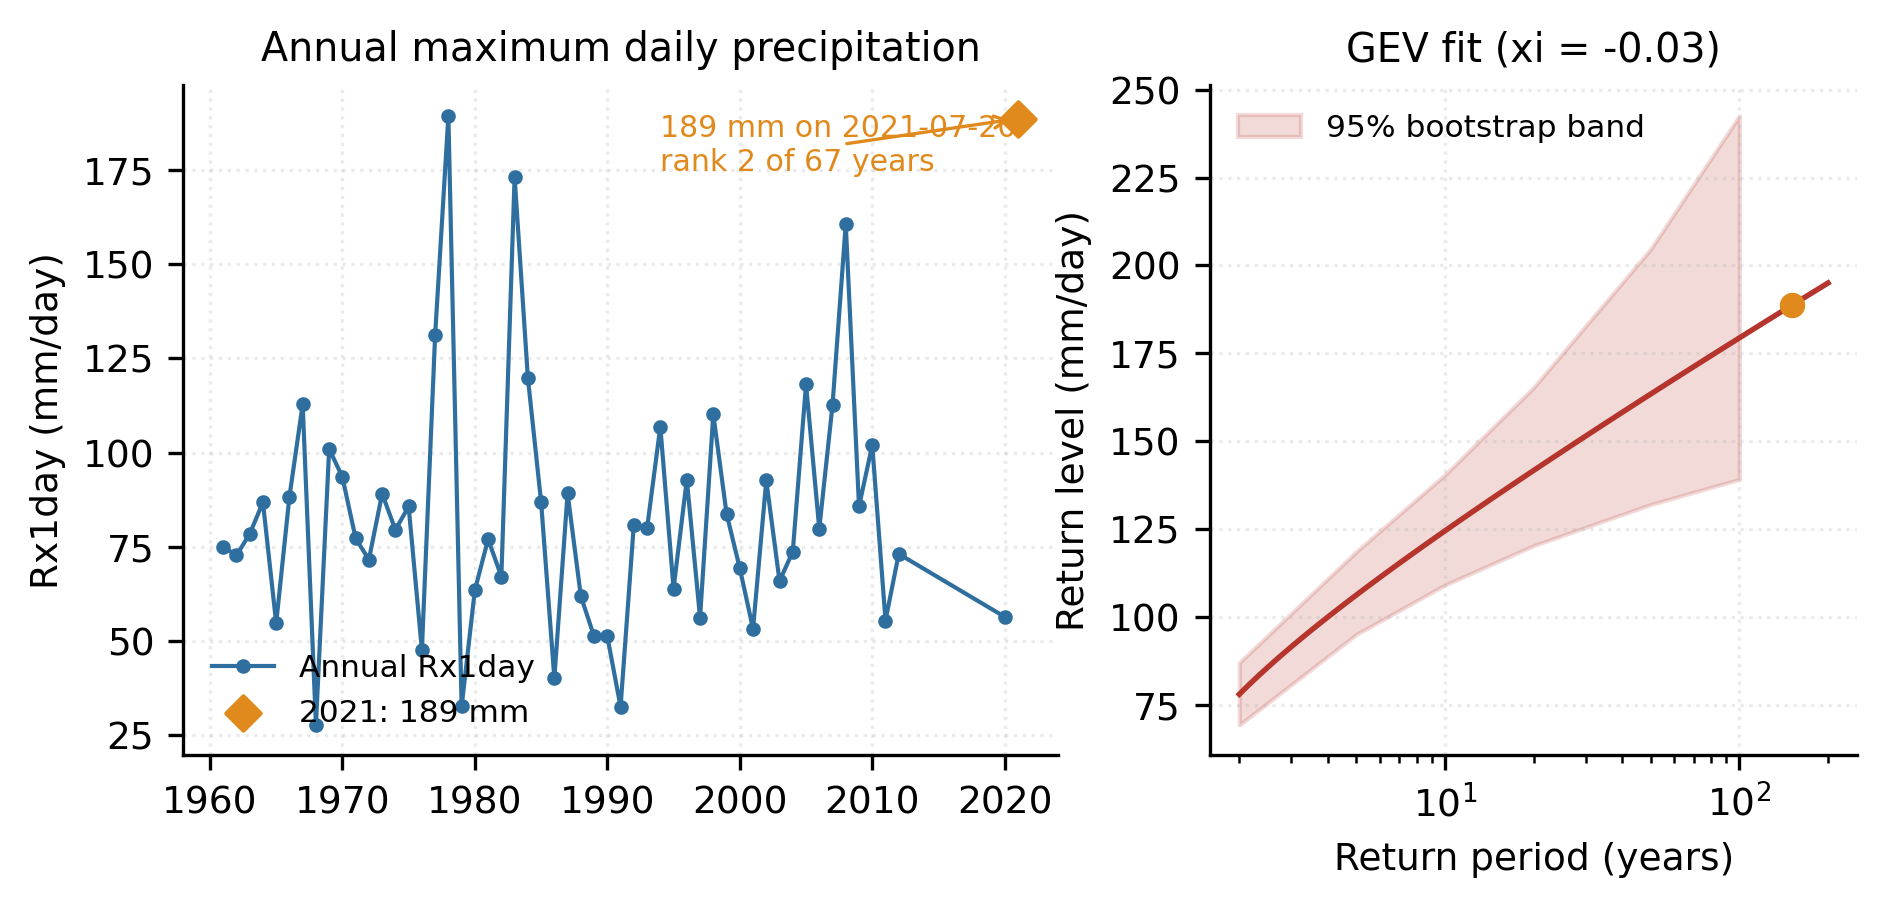
\includegraphics[width=0.62\linewidth]{../02_figures/fig02_rx1day_gev.png}
\caption{Annual maximum one-day rainfall at Zhengzhou with the fitted GEV curve; the 2021 value (188.7\,mm, marker) sits above the 100-year level of 179.4\,mm.}
\label{fig:rx1day}
\end{figure}

\begin{figure}[H]
\centering
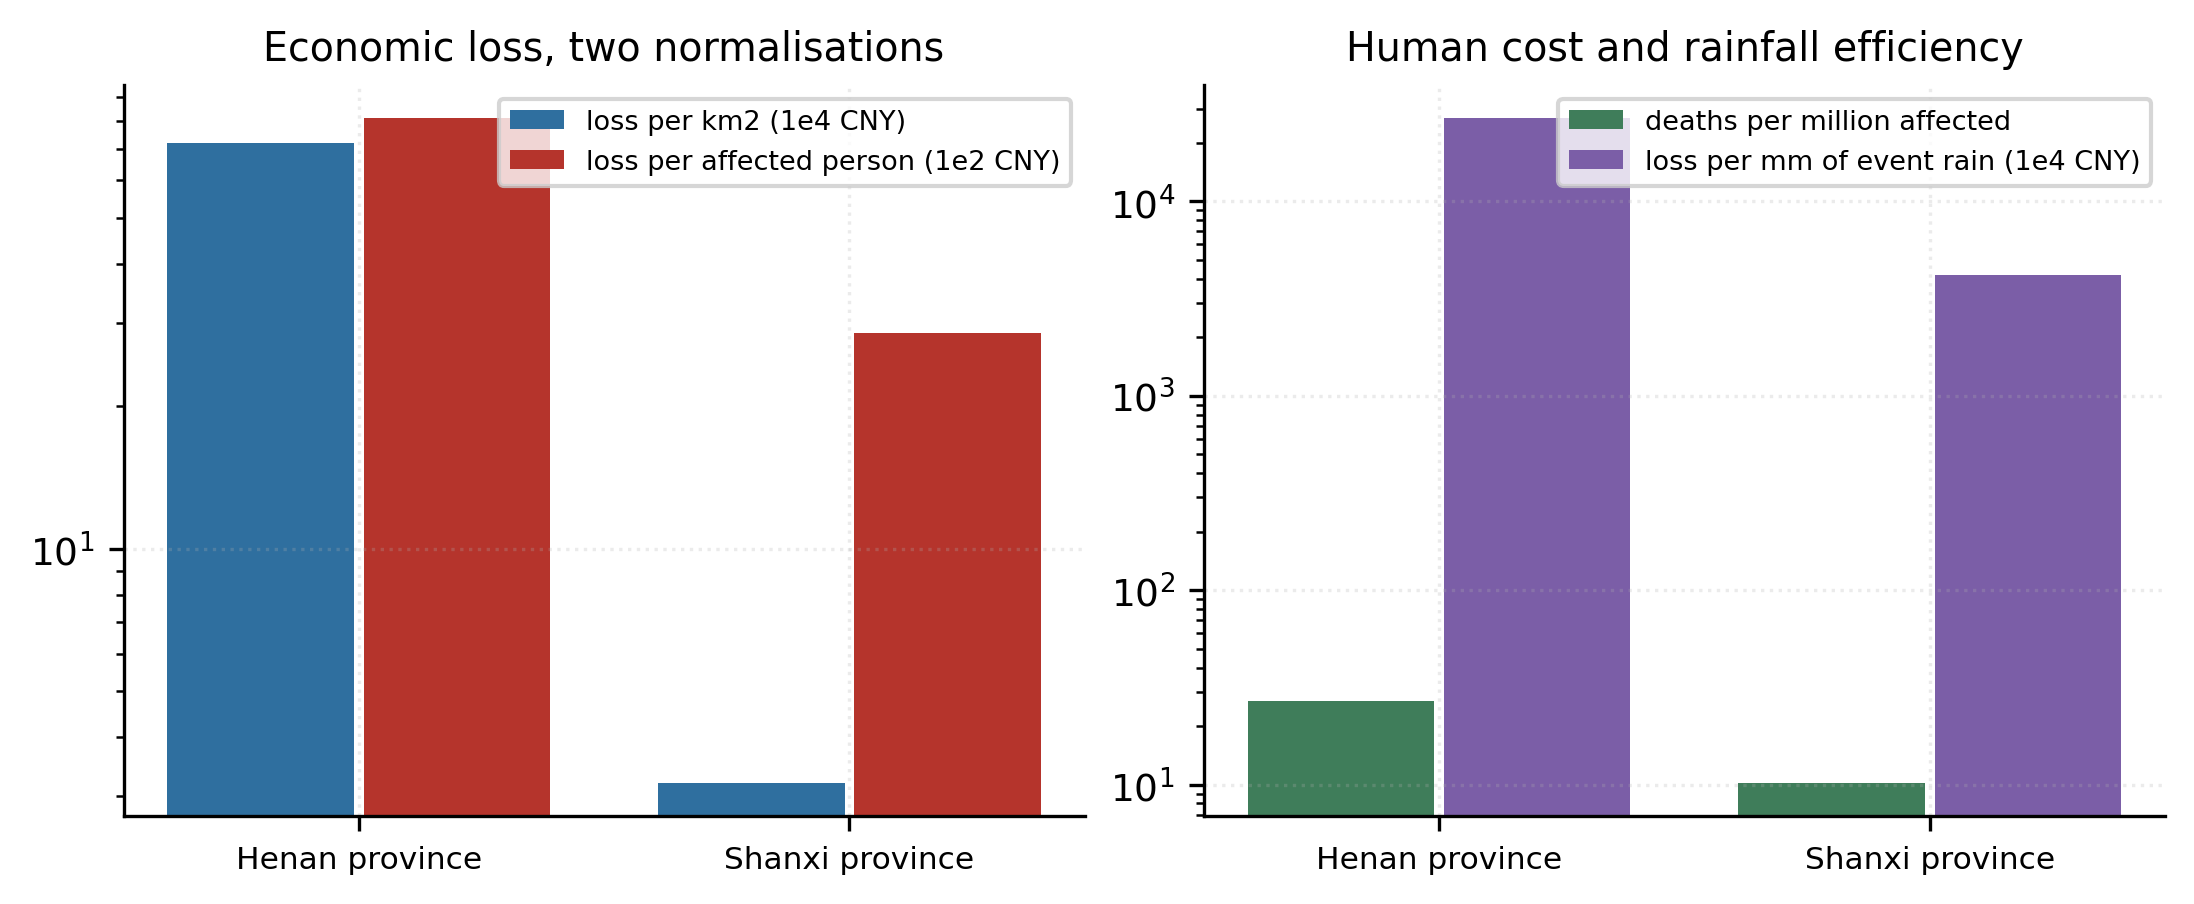
\includegraphics[width=0.62\linewidth]{../02_figures/fig19_loss_normalised.png}
\caption{Two normalisations of the loss. Left: loss per km$^2$ and loss per affected person. Right: deaths per million affected and loss per mm of event rainfall; the two rainfall denominators differ (the official 449\,mm areal total for Henan, a province-wide four-day mean for Shanxi), so that bar is indicative only.}
\label{fig:lossnorm}
\end{figure}

\begin{figure}[H]
\centering
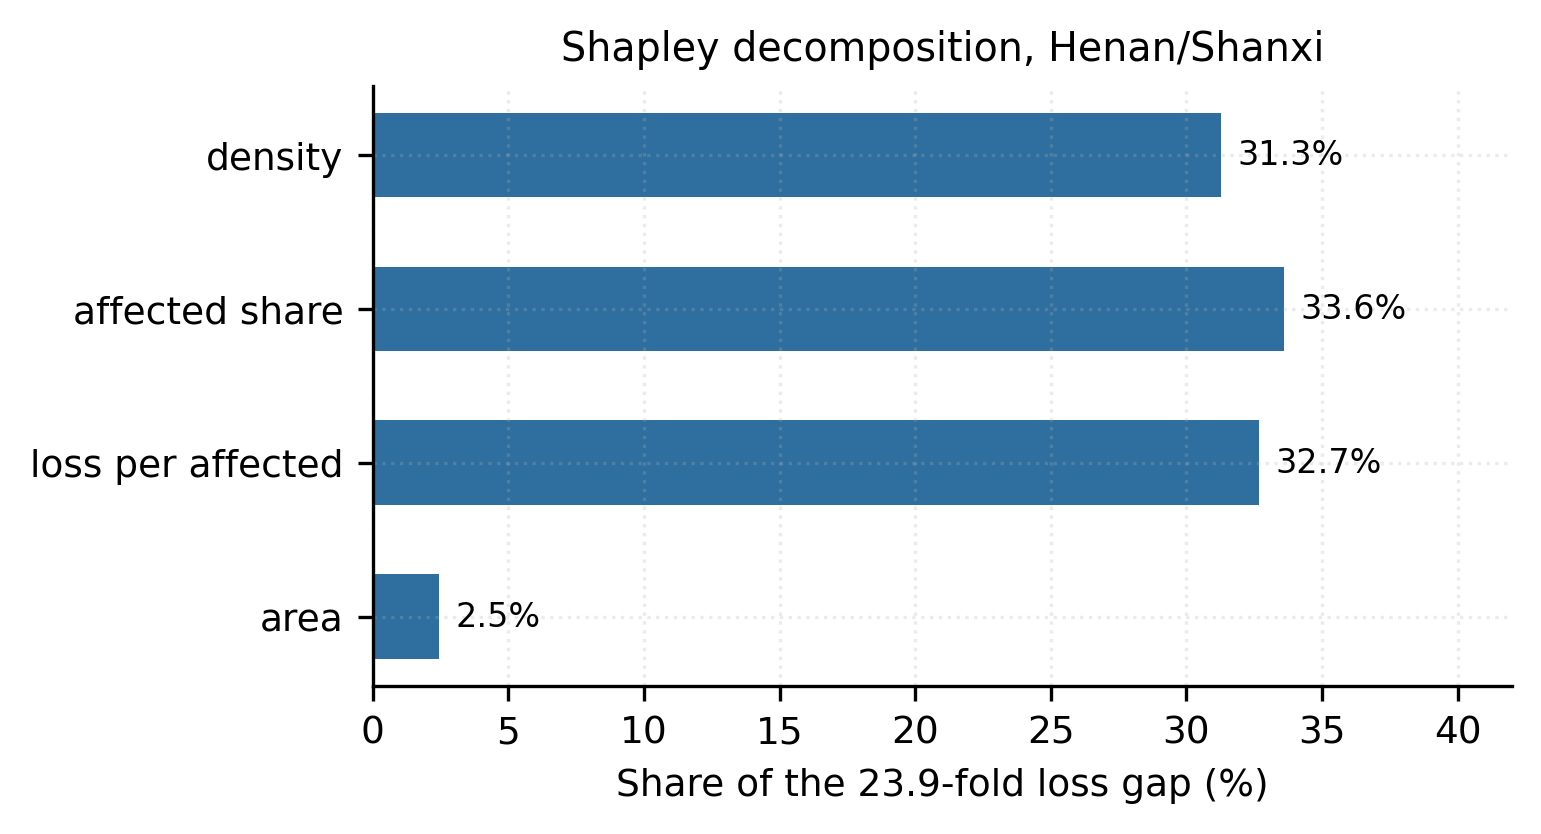
\includegraphics[width=0.58\linewidth]{../02_figures/fig24_q4_shapley.png}
\caption{Shapley shares of the 23.9-fold loss gap between Henan and Shanxi, with the four factors as players and partial products as coalition worth. Density, affected share and loss per affected person divide the gap almost equally; area contributes $2.5\%$.}
\label{fig:shapley}
\end{figure}

\begin{figure}[H]
\centering
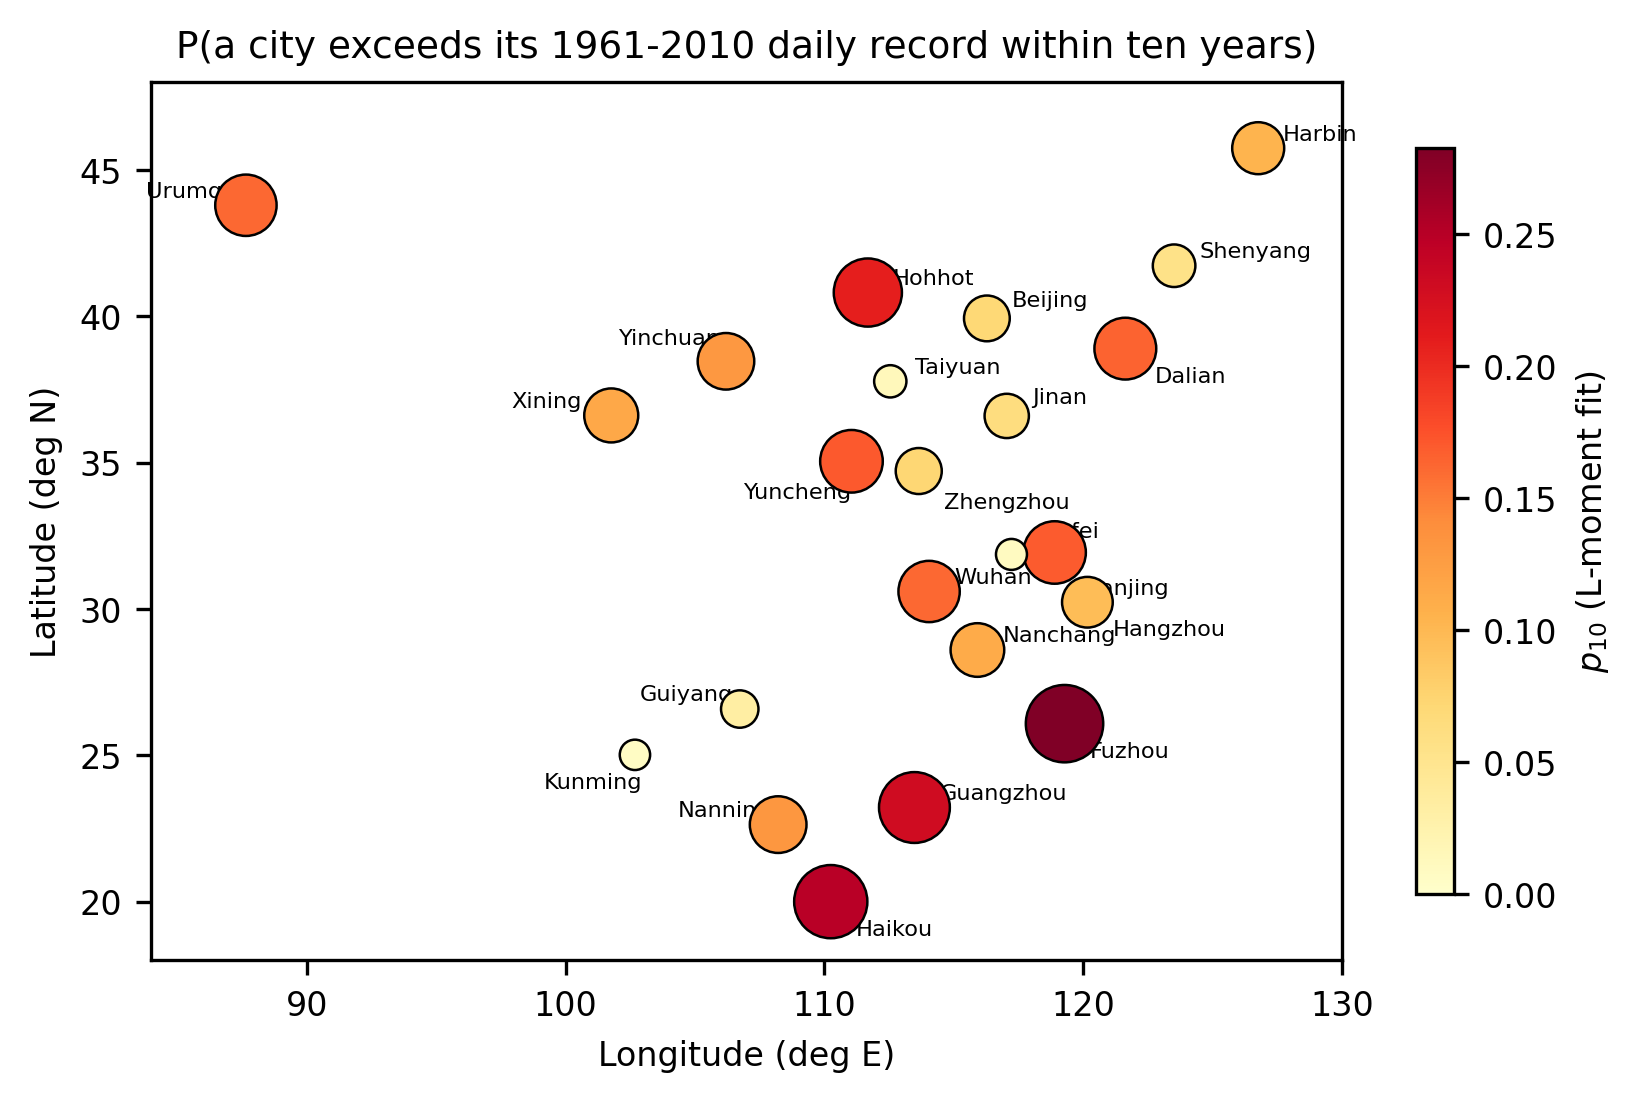
\includegraphics[width=0.62\linewidth]{../02_figures/fig14_risk_map.png}
\caption{Ten-year probability $p_{10}$ of exceeding the 1961--2010 daily record for the 23 cities, from the L-moment fit; the marker area is proportional to $p_{10}$.}
\label{fig:riskmap}
\end{figure}

\begin{figure}[H]
\centering
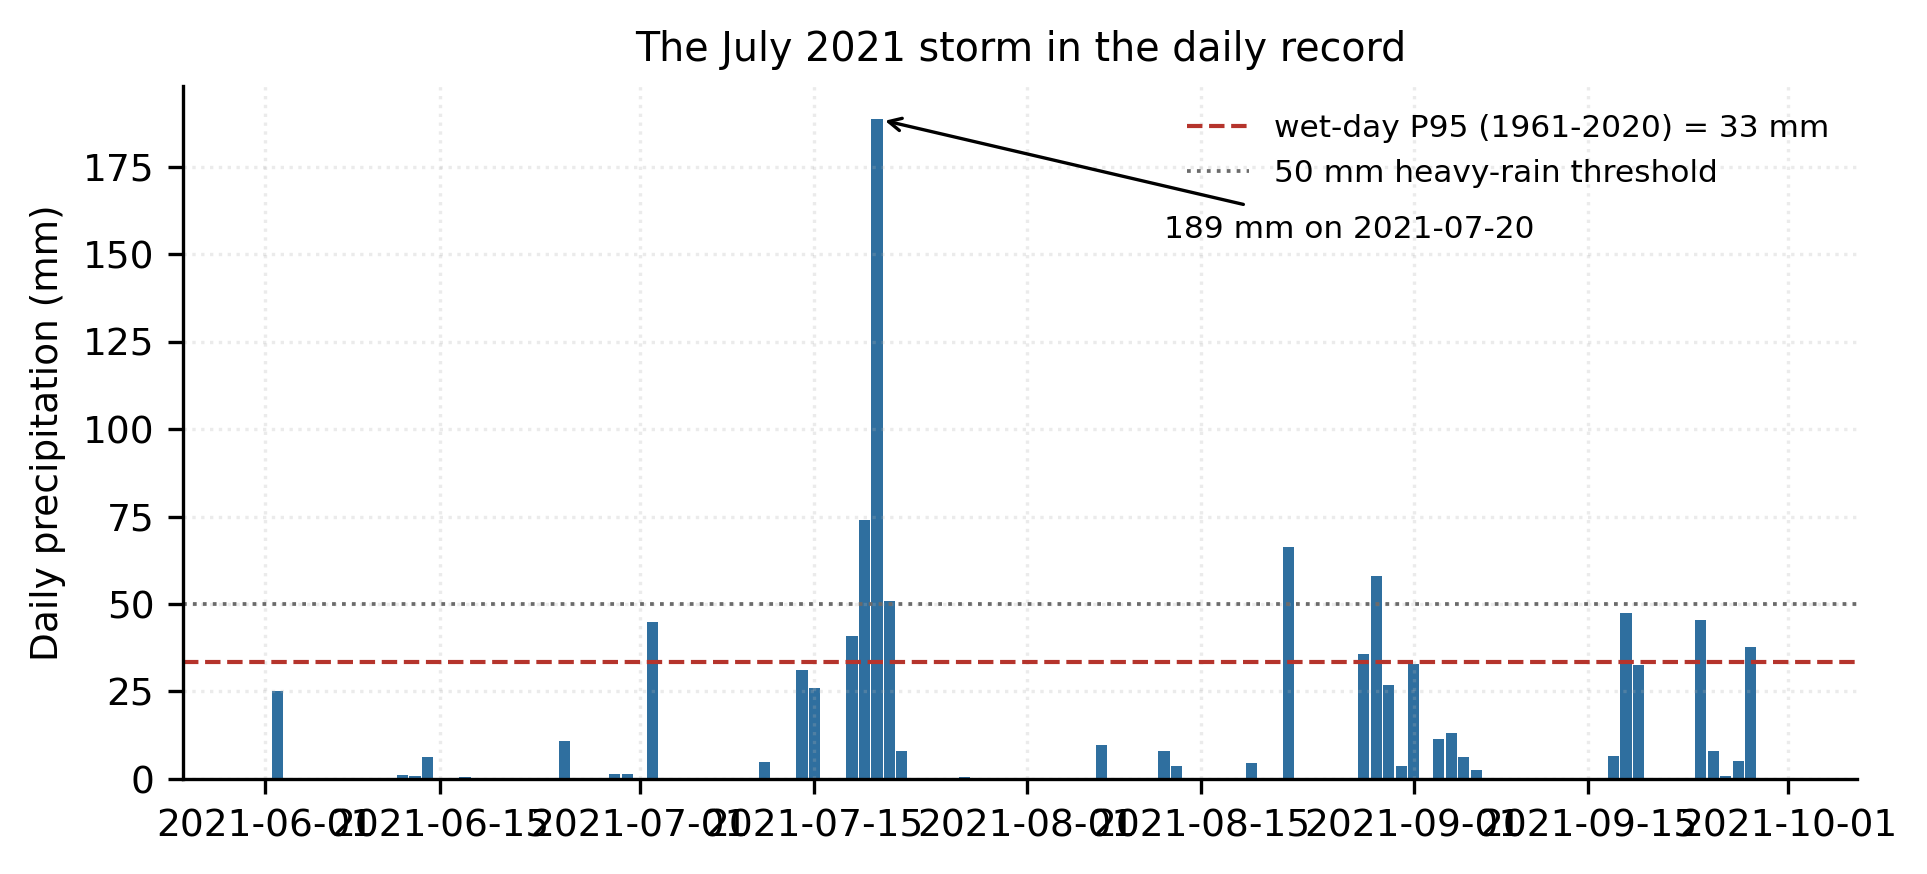
\includegraphics[width=0.62\linewidth]{../02_figures/fig05_event_profile.png}
\caption{The July 2021 storm in the daily record (1 June--30 September 2021). Dashed red line: wet-day 95th percentile of 1961--2020; dotted grey line: the 50\,mm heavy-rain threshold; the annotated bar is 188.7\,mm on 20 July.}
\label{fig:profile}
\end{figure}

\begin{figure}[H]
\centering
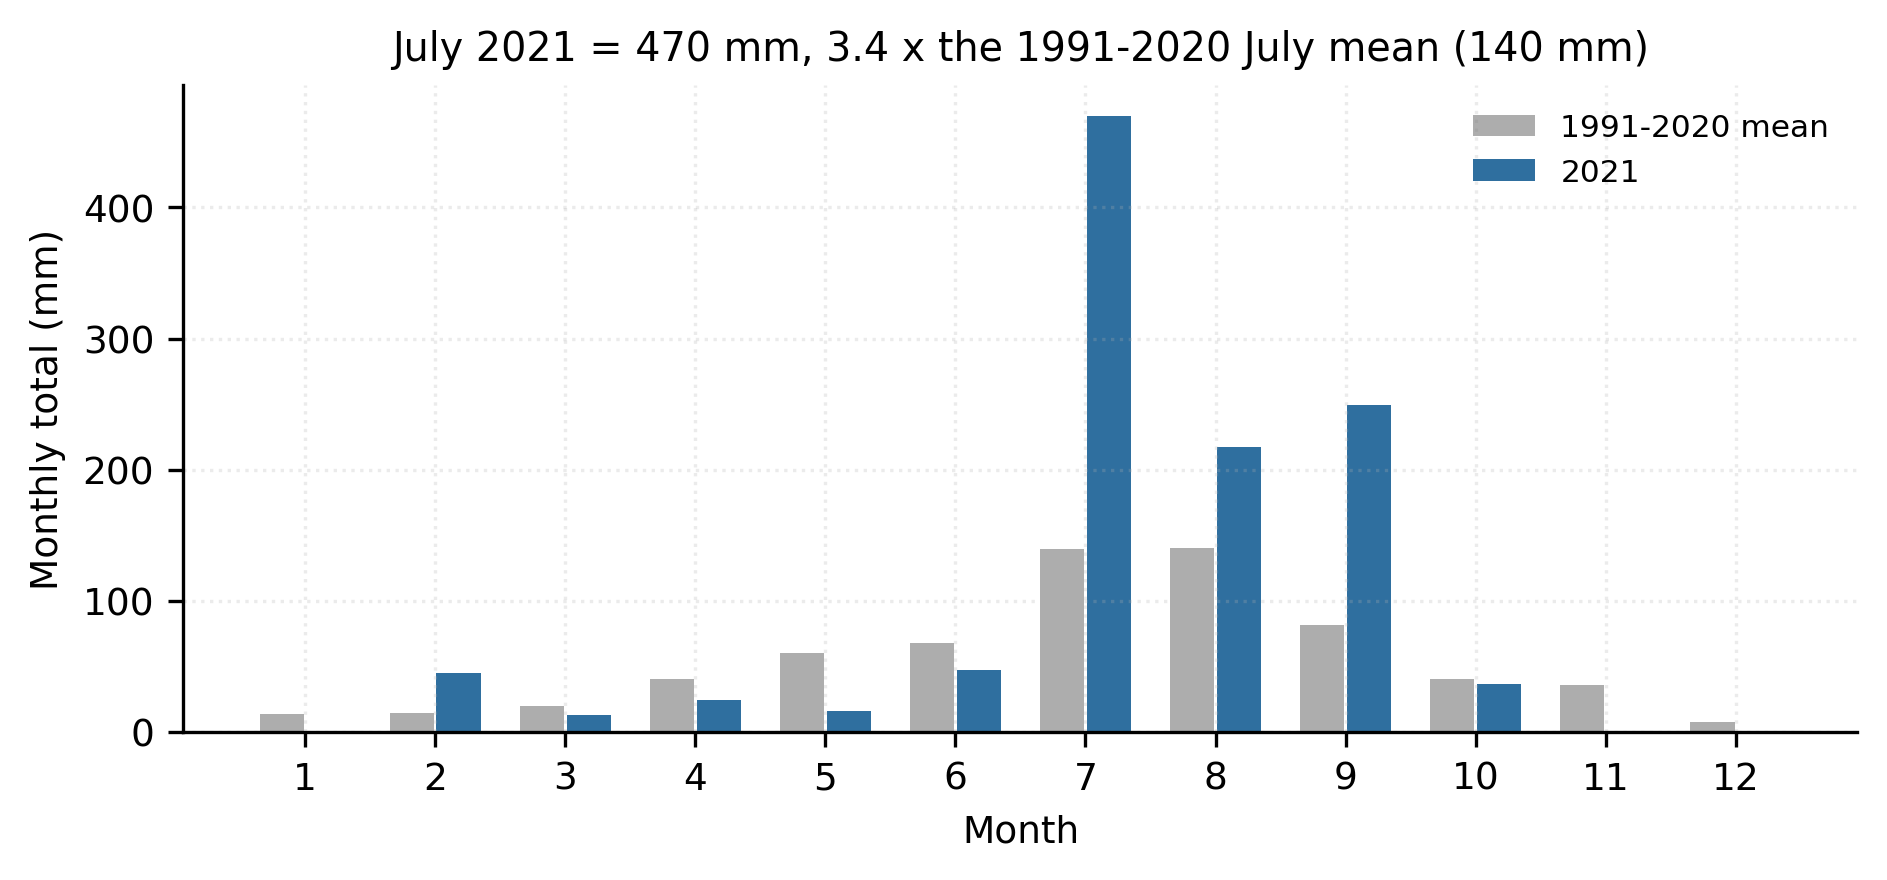
\includegraphics[width=0.62\linewidth]{../02_figures/fig03_monthly_2021.png}
\caption{Monthly totals in 2021 against the 1991--2020 monthly means. July 2021 reached 469.6\,mm, 3.4 times the July normal of 139.8\,mm.}
\end{figure}

\begin{figure}[H]
\centering
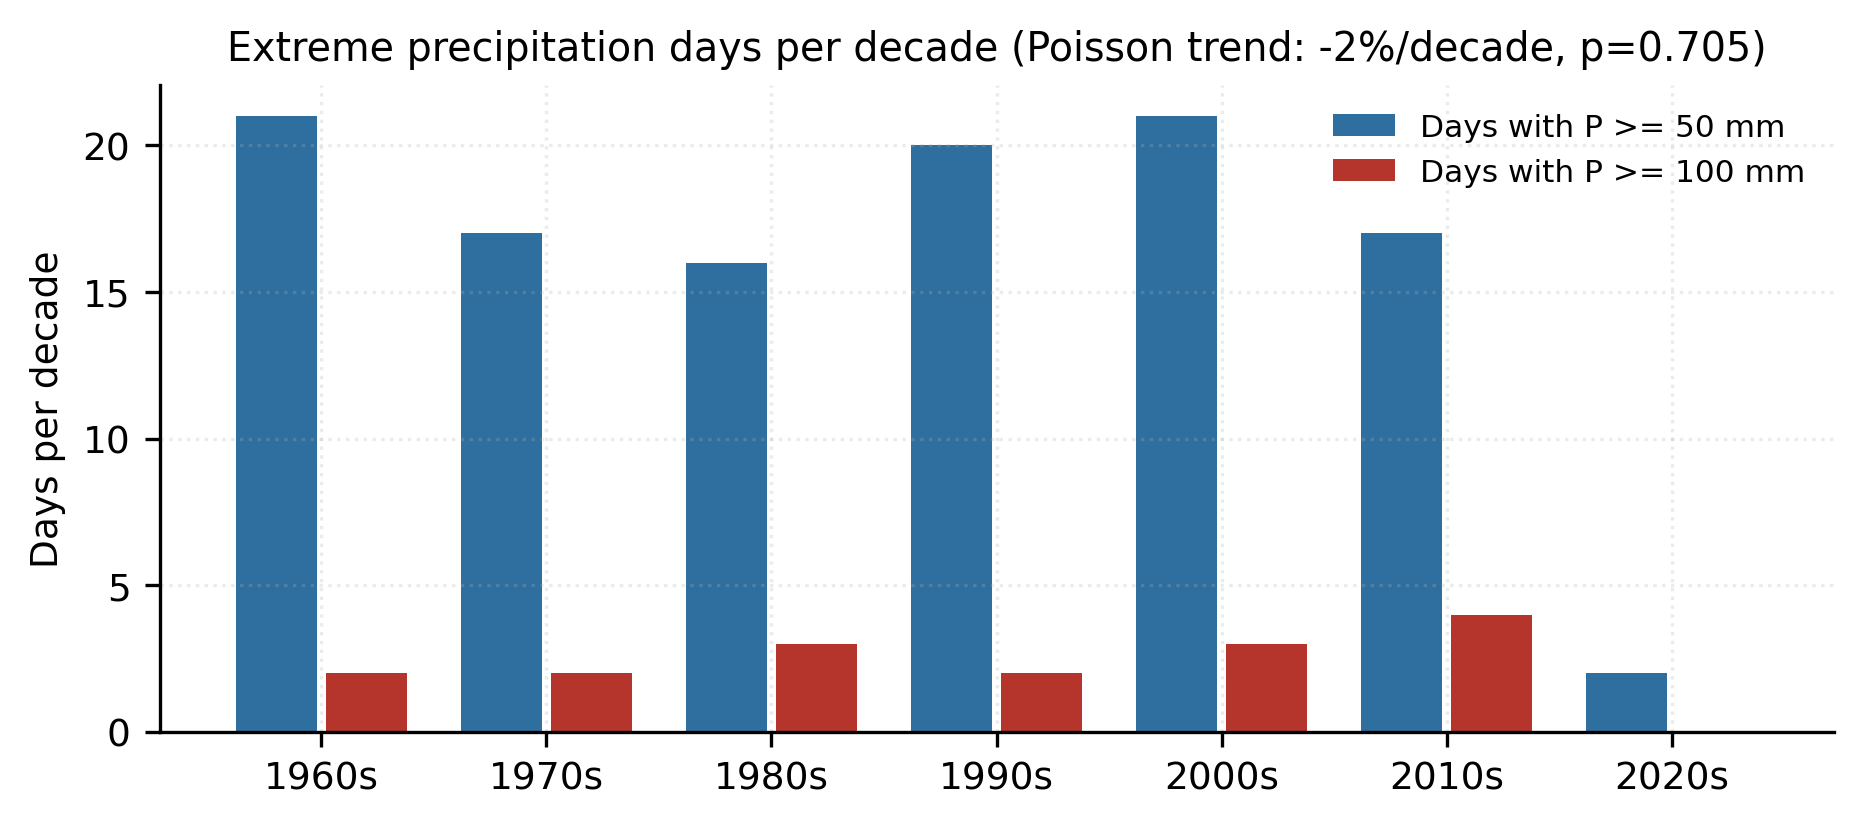
\includegraphics[width=0.62\linewidth]{../02_figures/fig04_extreme_days.png}
\caption{Decadal counts of days with precipitation above 50\,mm and above 100\,mm at Zhengzhou. The Poisson trend for days above 50\,mm is $-2.0\%$ per decade ($p=0.705$).}
\end{figure}

\begin{figure}[H]
\centering
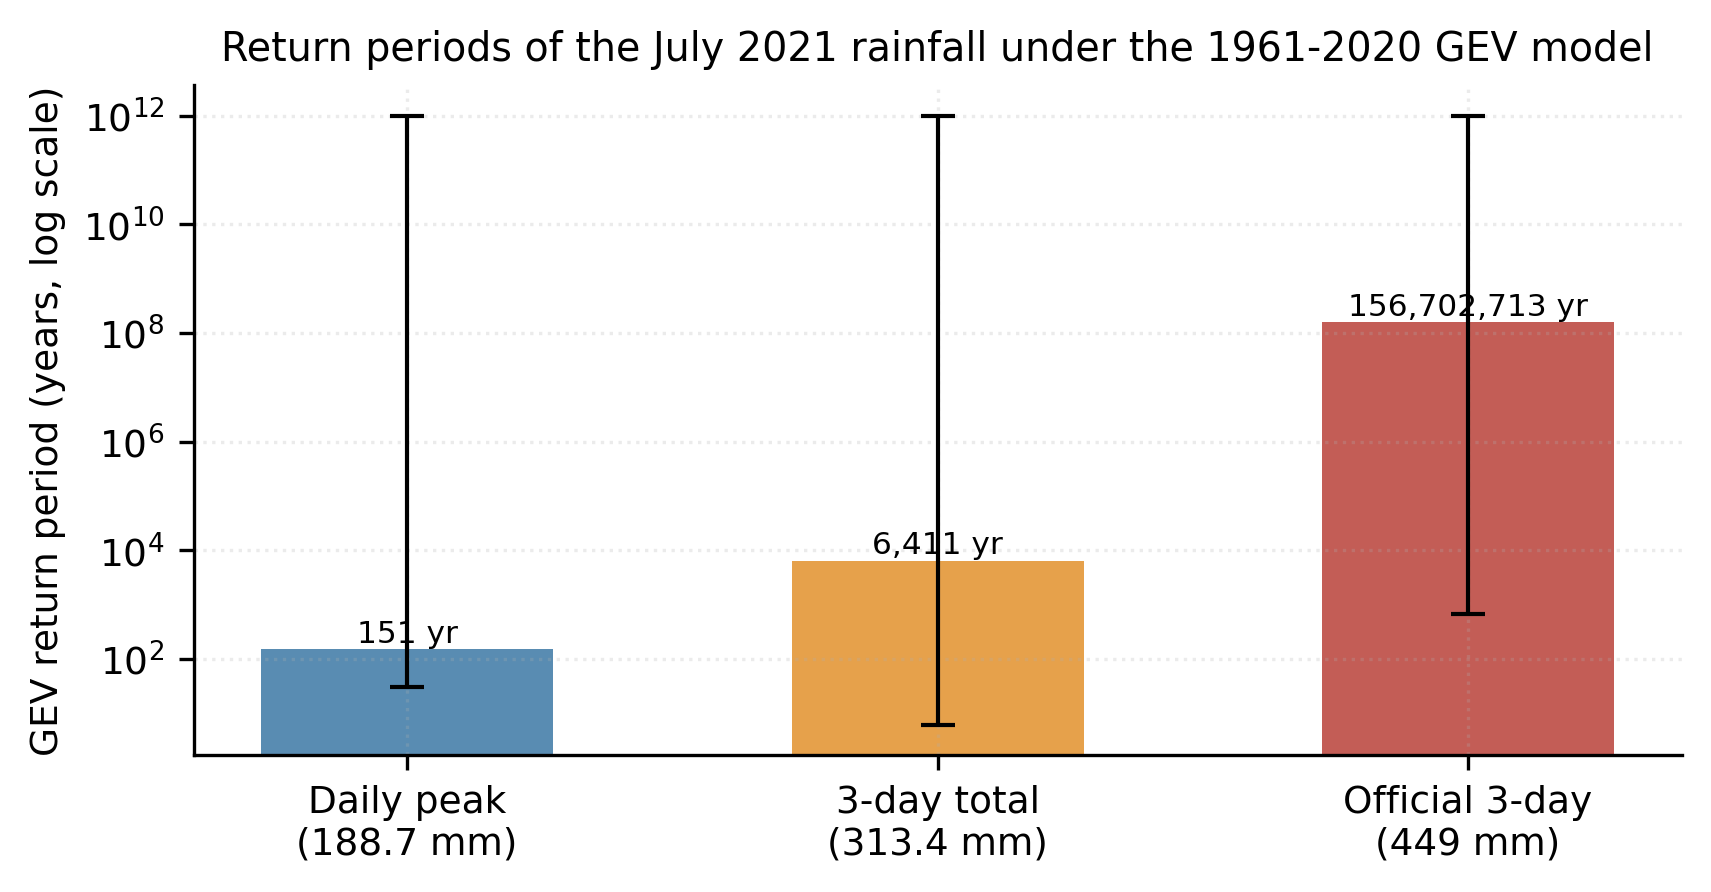
\includegraphics[width=0.58\linewidth]{../02_figures/fig06_event_return_periods.png}
\caption{Return periods of the three rainfall metrics of the July 2021 event on a logarithmic axis, with bootstrap intervals. The interval for the official 449\,mm total extends beyond the plotted range.}
\end{figure}

\begin{figure}[H]
\centering
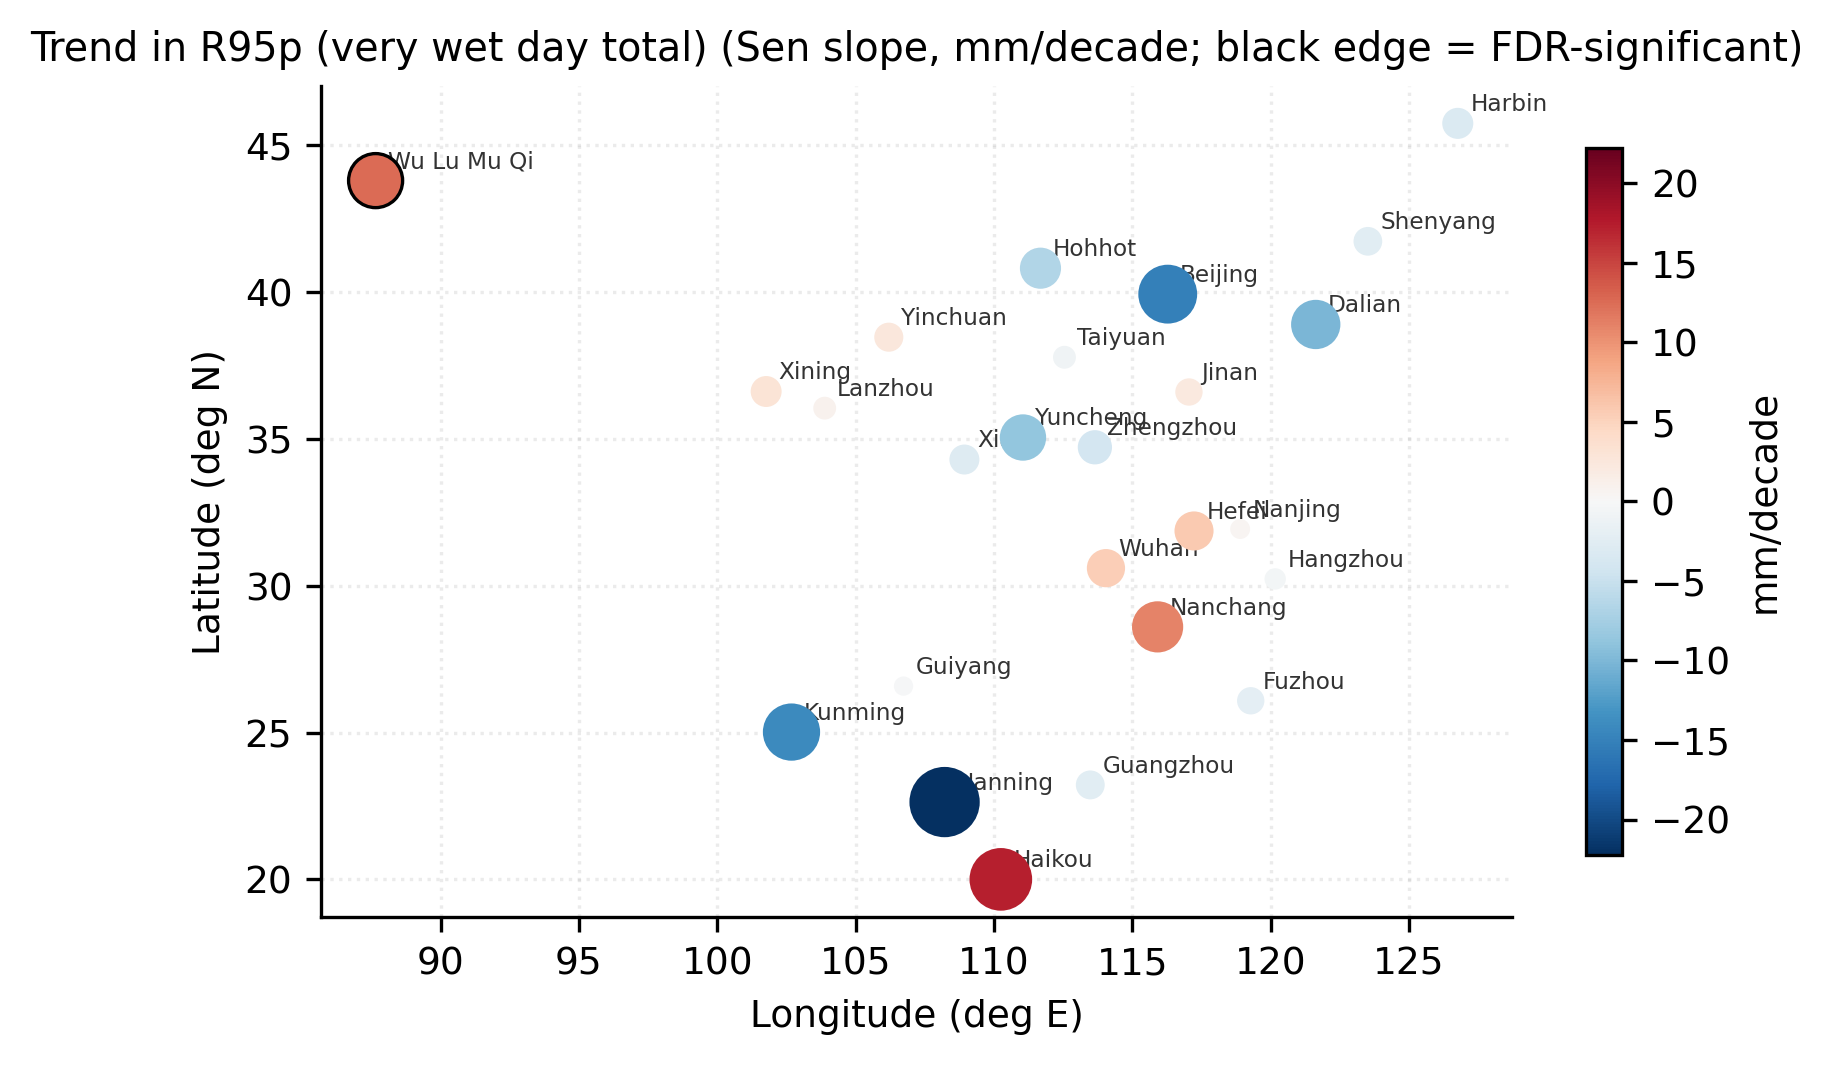
\includegraphics[width=0.62\linewidth]{../02_figures/fig08_trend_map_r95p.png}
\caption{Sen slope of annual R95p (mm per decade) for the national panel; red denotes increasing extreme-rainfall totals.}
\end{figure}

\begin{figure}[H]
\centering
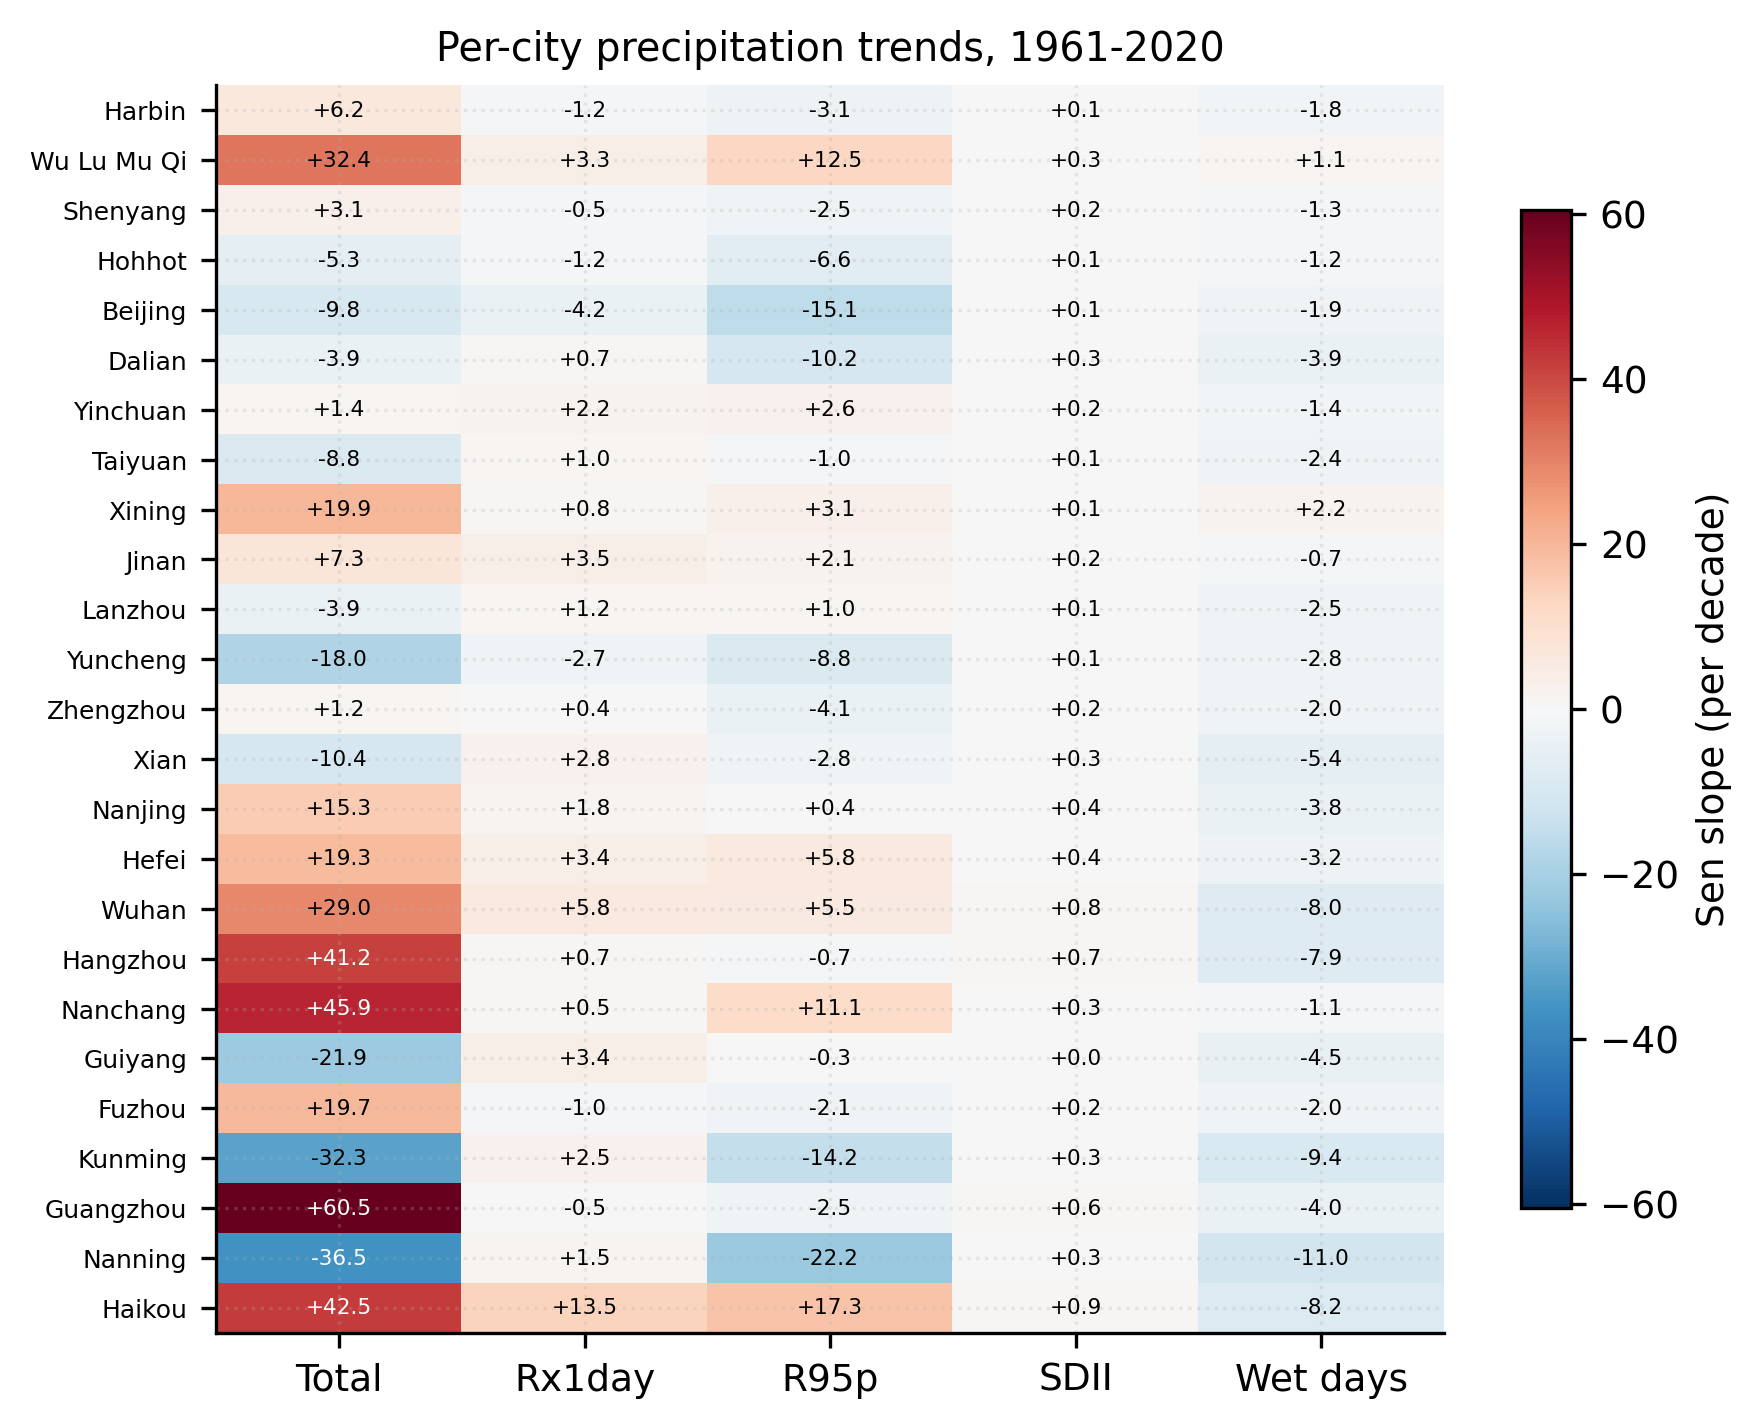
\includegraphics[width=0.62\linewidth]{../02_figures/fig09_trend_heatmap.png}
\caption{City-by-index matrix of Sen slopes, ordered by cluster. Colour is the standardised slope; blank cells are indices with fewer than 45 valid years.}
\end{figure}

\begin{figure}[H]
\centering
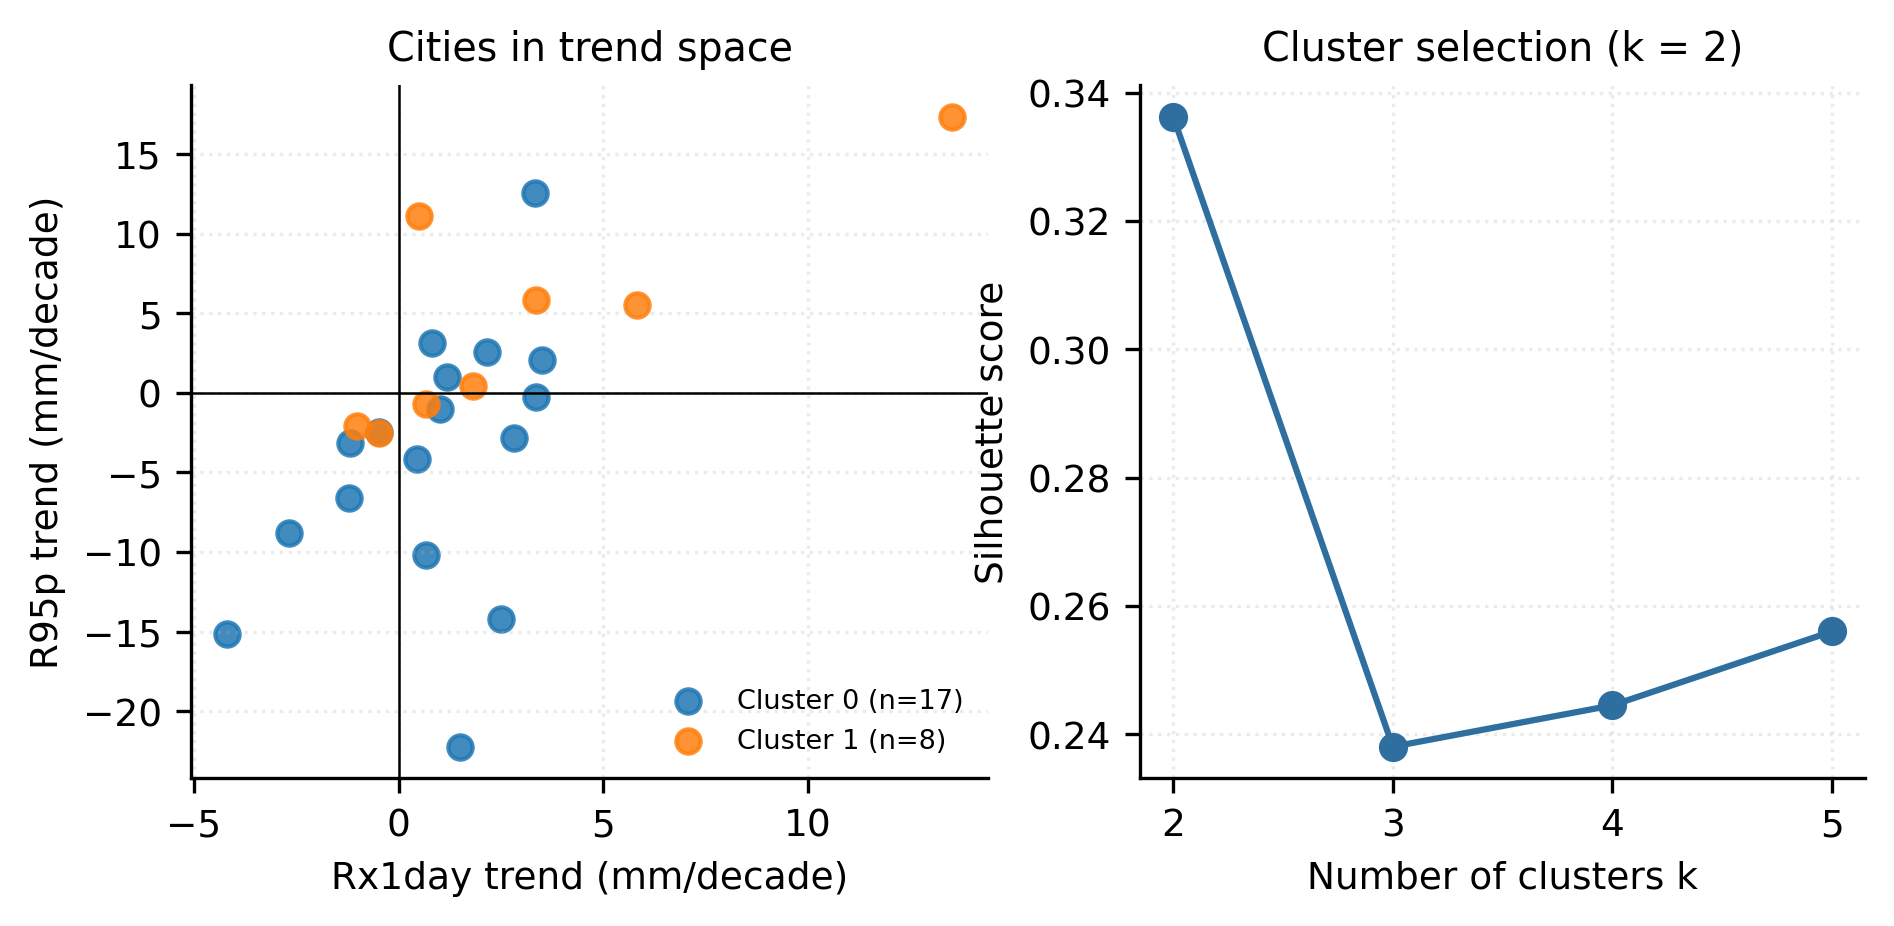
\includegraphics[width=0.56\linewidth]{../02_figures/fig10_clusters.png}
\caption{$k$-means partition of the 25 cities in the space of the first two standardised trend components, with cluster centroids. Silhouette scores: $k=2$, 0.336; $k=3$, 0.238.}
\end{figure}

\begin{figure}[H]
\centering
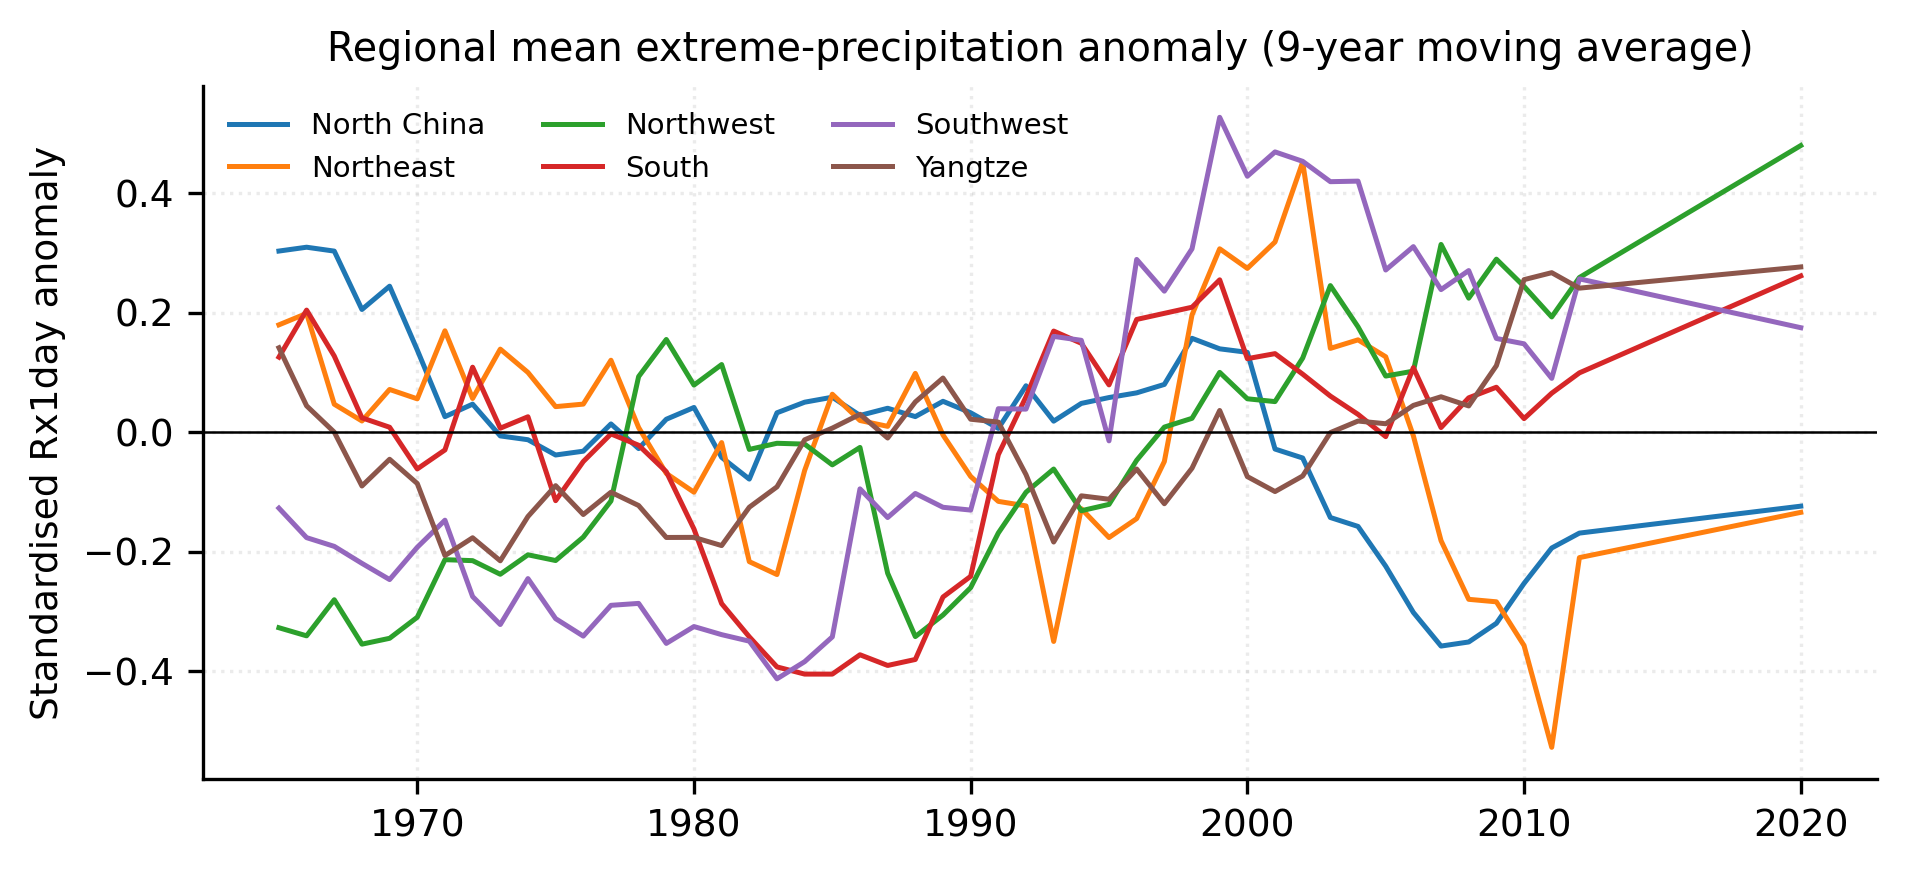
\includegraphics[width=0.62\linewidth]{../02_figures/fig11_regional_anomaly.png}
\caption{Regional standardised anomalies of annual precipitation, smoothed with a five-year running mean. The divergence after 1990 is the regional structure discussed in Section~\ref{sec:q2}.}
\end{figure}

\begin{figure}[H]
\centering
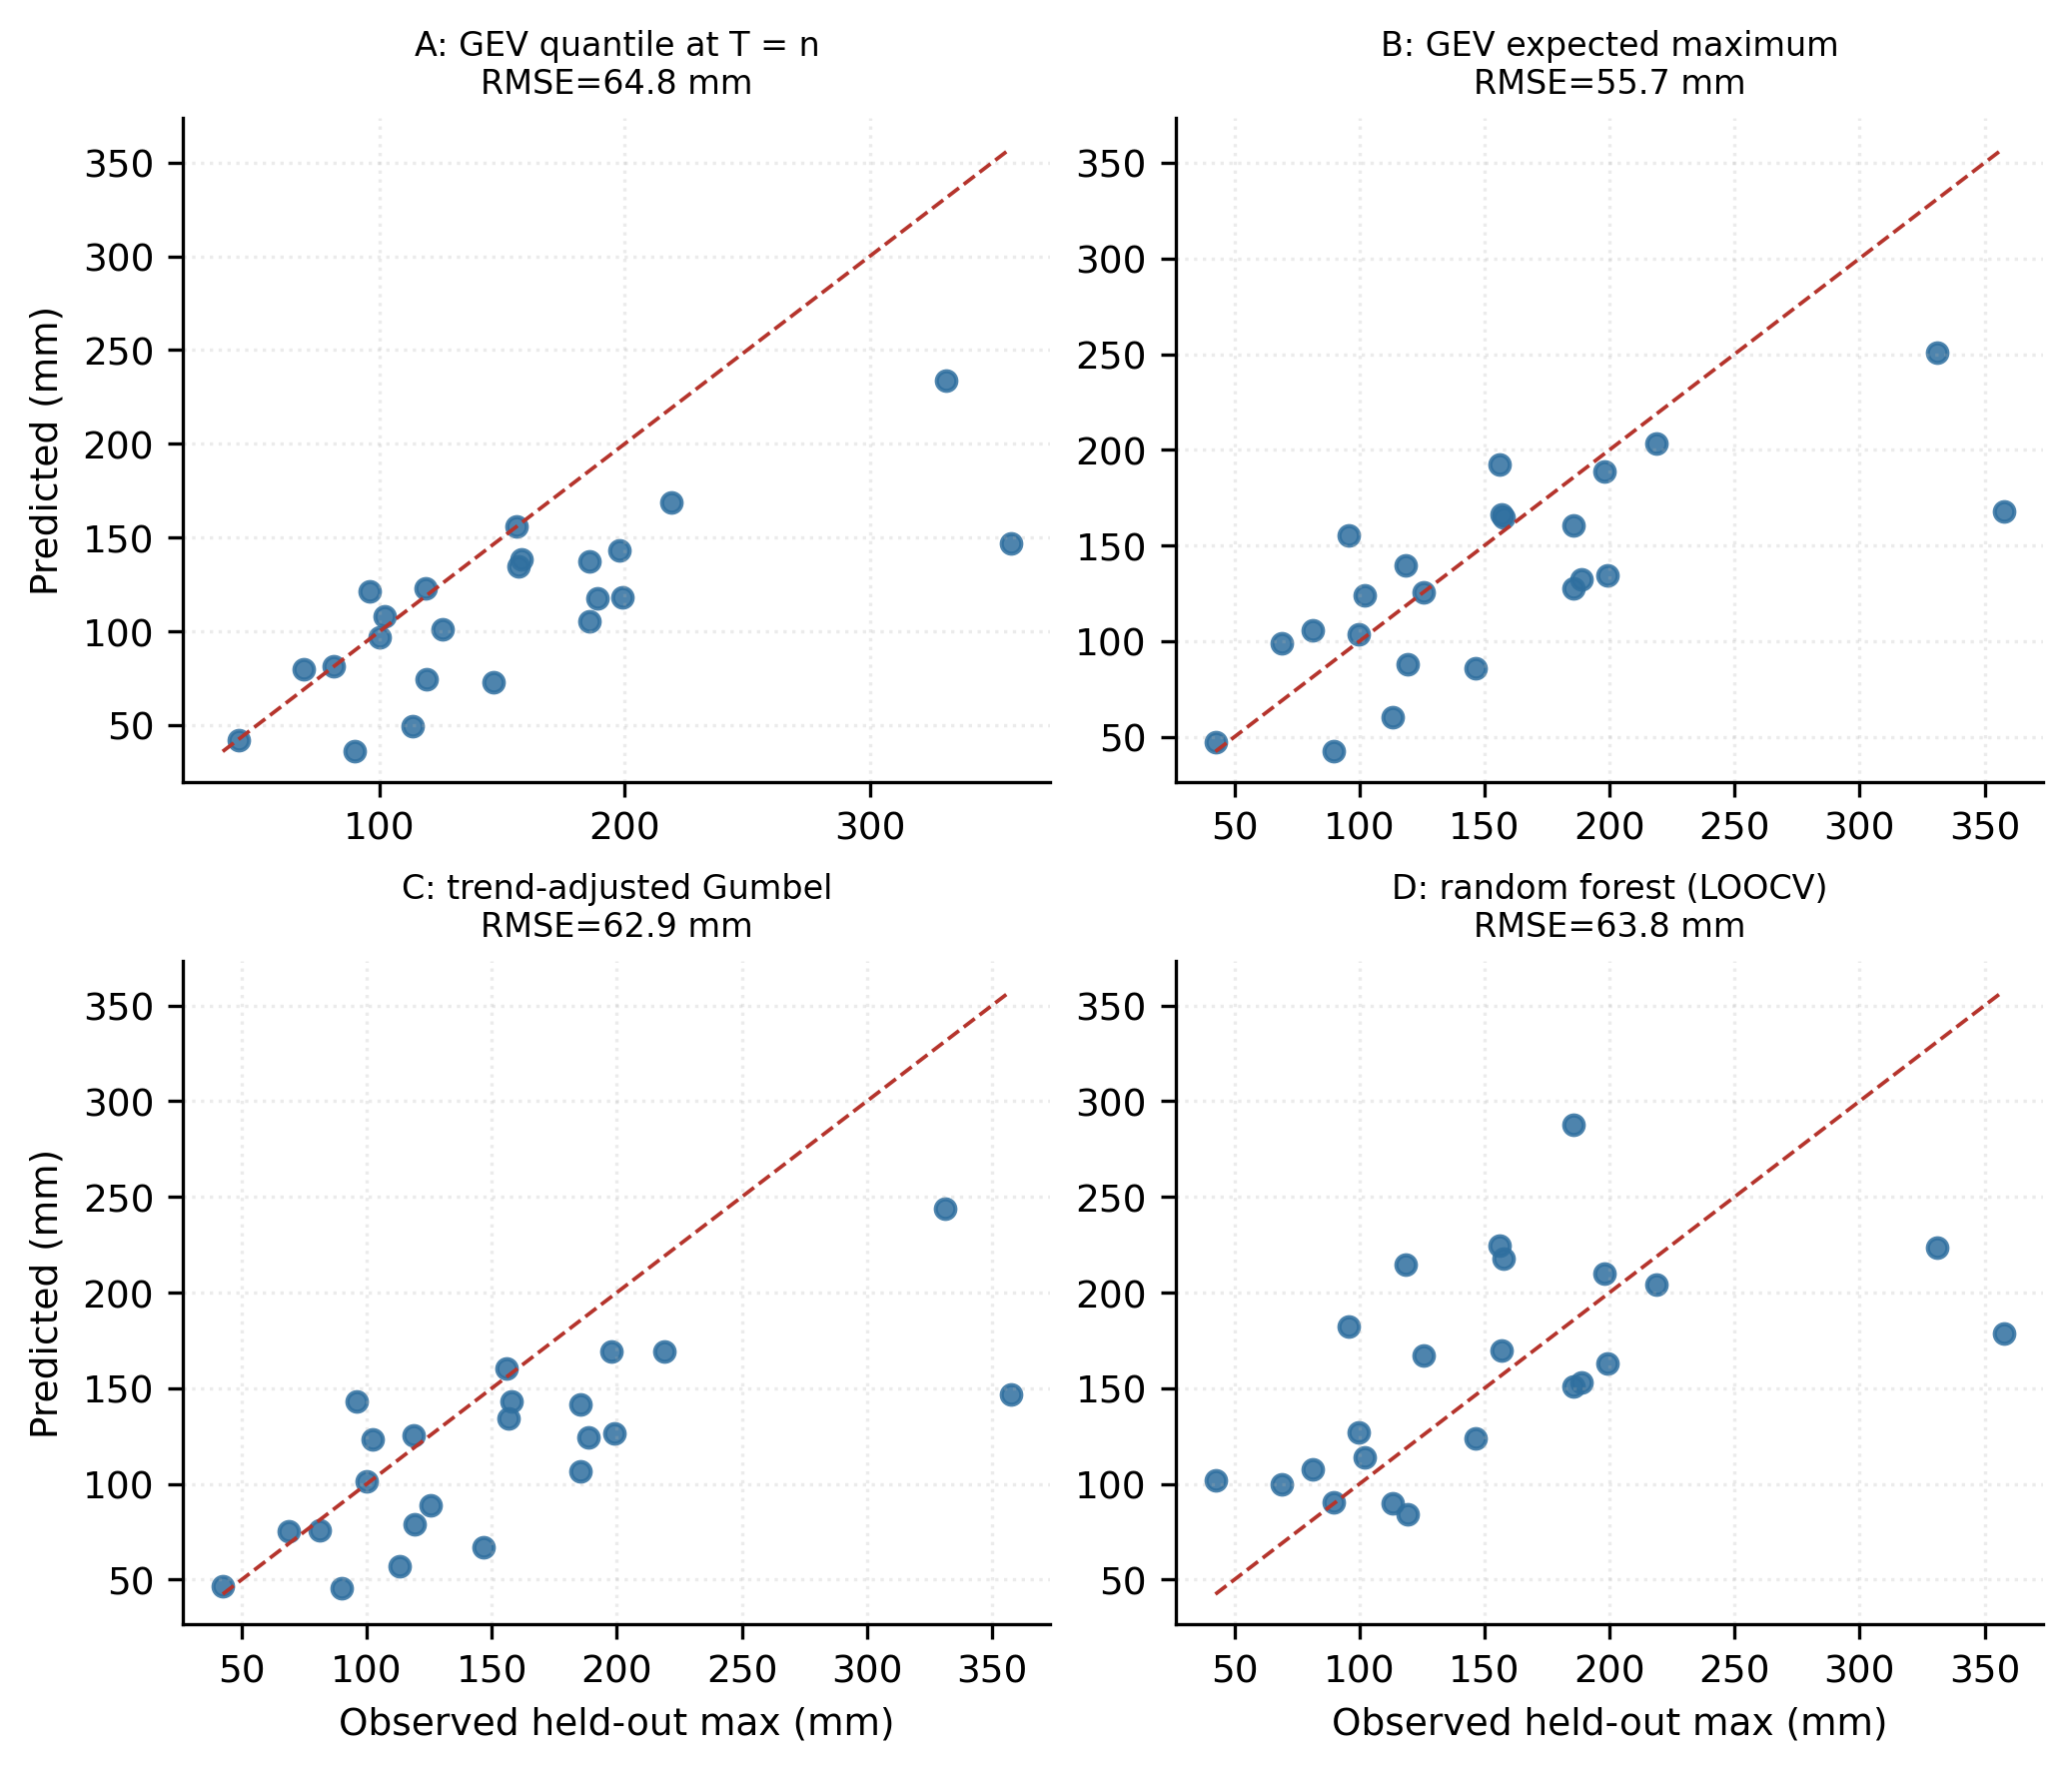
\includegraphics[width=0.62\linewidth]{../02_figures/fig12_method_scatter.png}
\caption{Predicted versus observed held-out maxima for four representative methods. The diagonal is perfect prediction; the horizontal offset of the cloud is the definitional bias of the quantile target.}
\end{figure}

\begin{figure}[H]
\centering
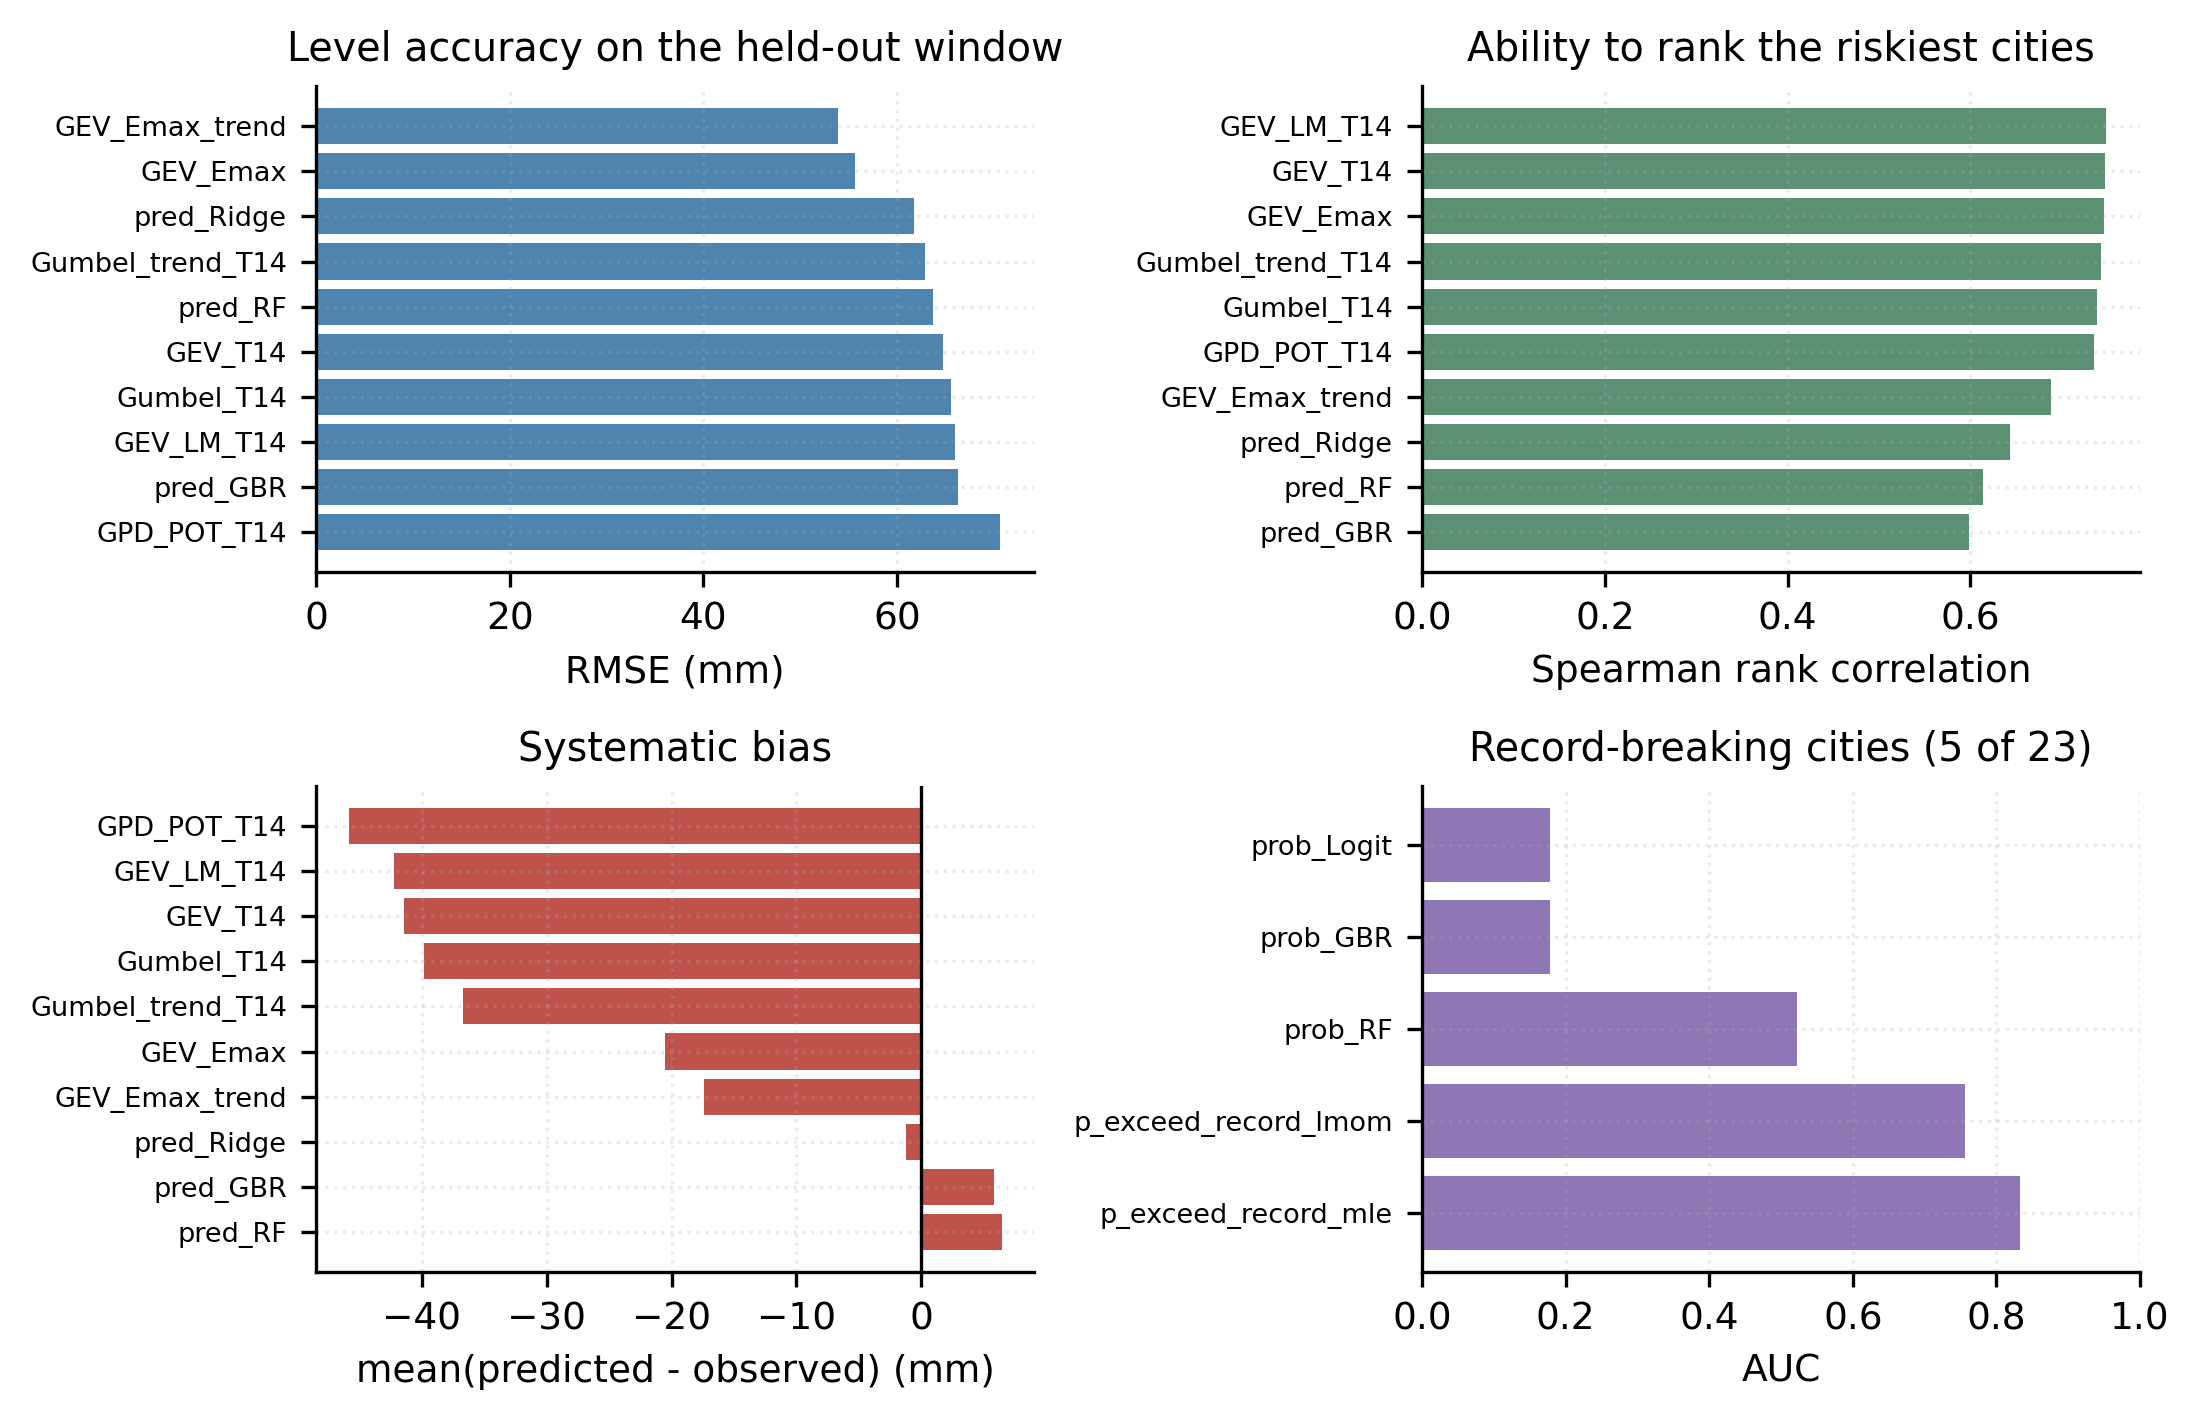
\includegraphics[width=0.62\linewidth]{../02_figures/fig13_method_comparison.png}
\caption{Four criteria for the ten forecast strategies: RMSE, Spearman correlation, bias and, for the classification task, AUC.}
\end{figure}

\begin{figure}[H]
\centering
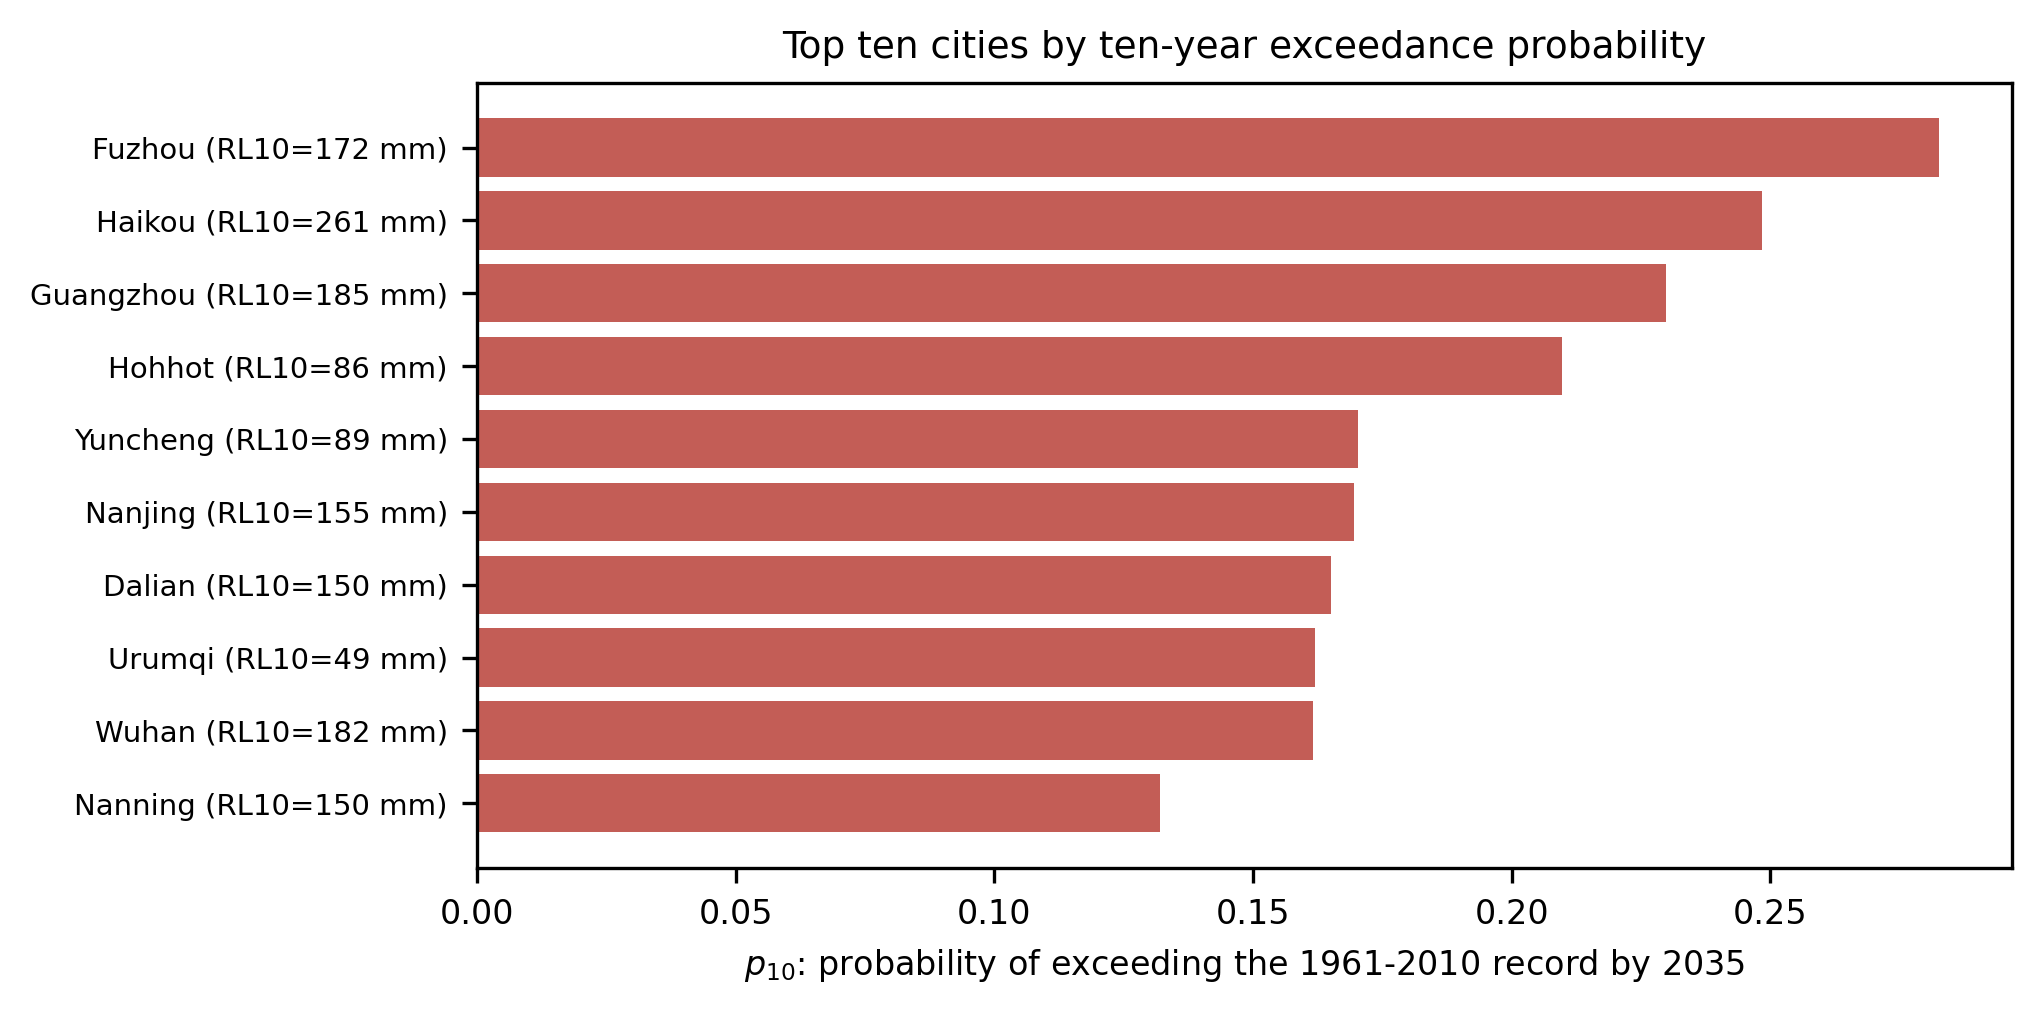
\includegraphics[width=0.58\linewidth]{../02_figures/fig15_risk_ranking.png}
\caption{Ten-year exceedance probability $p_{10}$ of the 1961--2010 record for the ten highest cities, with each city's L-moment ten-year return level in brackets.}
\end{figure}

\begin{figure}[H]
\centering
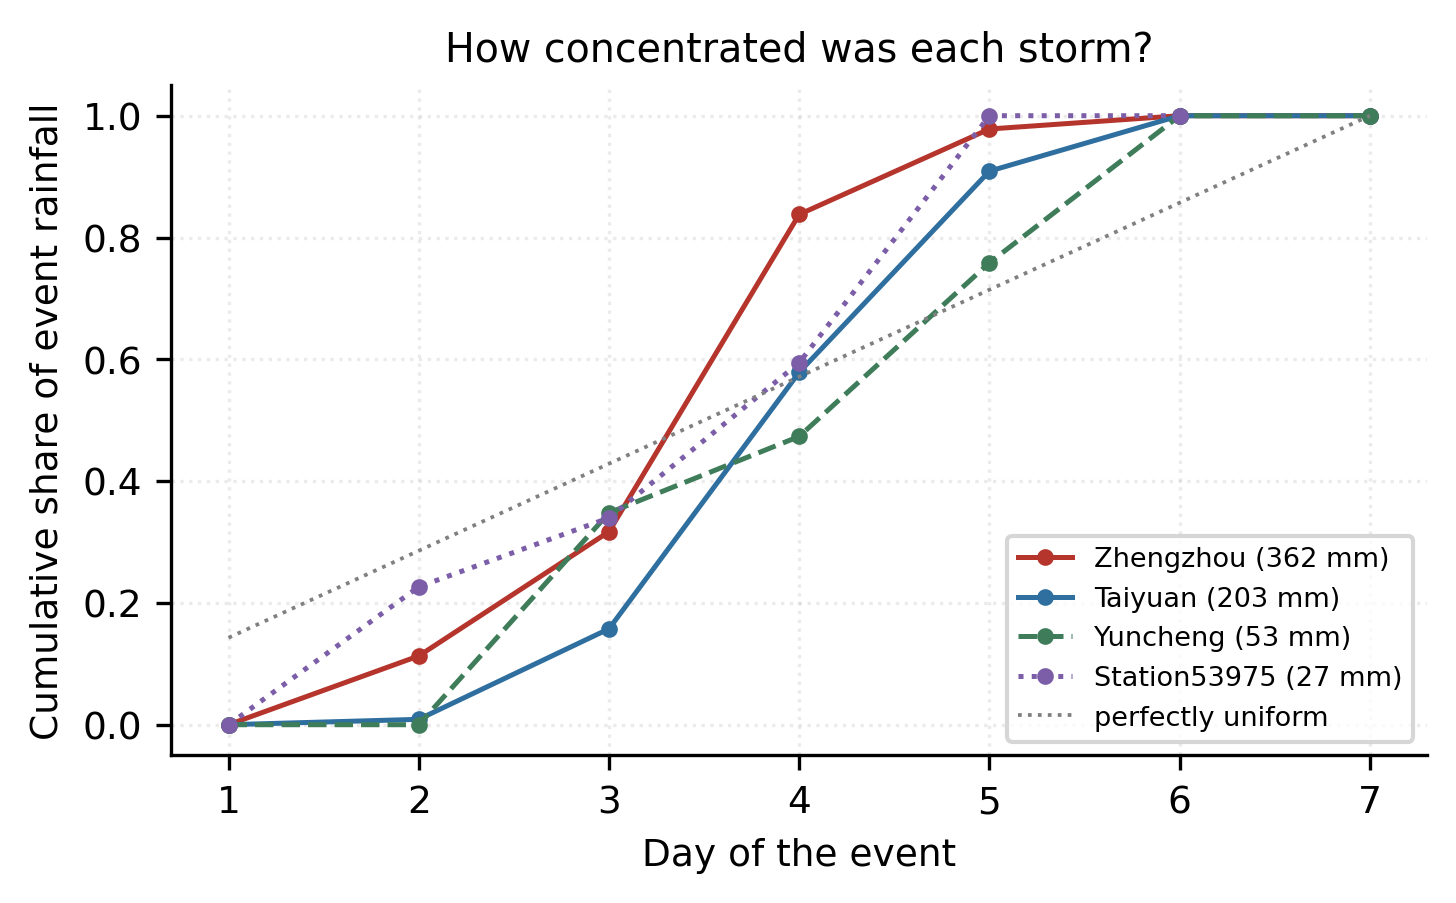
\includegraphics[width=0.62\linewidth]{../02_figures/fig17_concentration.png}
\caption{Cumulative share of event rainfall against elapsed time. The straight diagonal is a perfectly uniform event; Zhengzhou's curve is far above it, Taiyuan's close to it.}
\end{figure}

\begin{figure}[H]
\centering
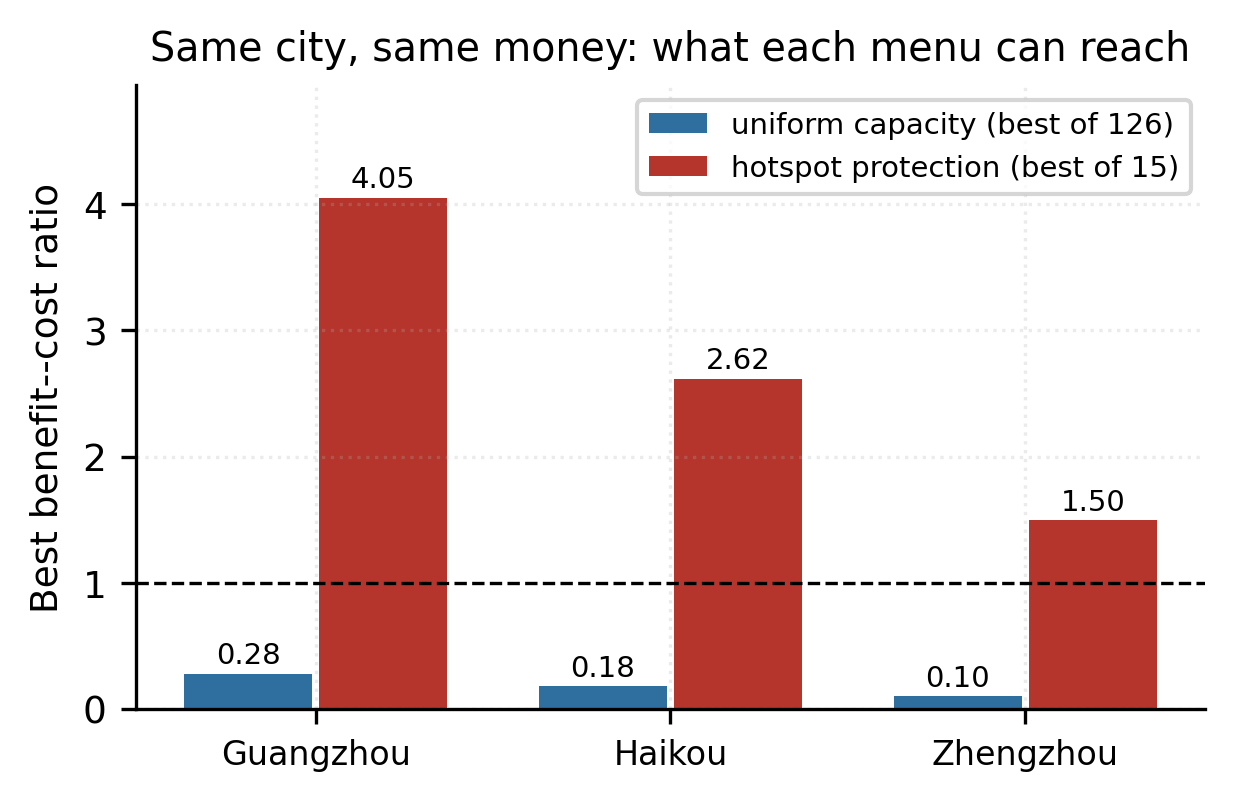
\includegraphics[width=0.60\linewidth]{../02_figures/fig21_bcr.png}
\caption{Best benefit--cost ratio reachable by each menu for the same city: uniform capacity over the 126-point design menu, and hotspot protection over the 15 assumed $(h,m)$ pairs at 5\,mm of local storage. The horizontal line is break-even; no uniform plan reaches it, while every city's hotspot plan does at the favourable pairs.}
\label{fig:bcr}
\end{figure}

\begin{figure}[H]
\centering
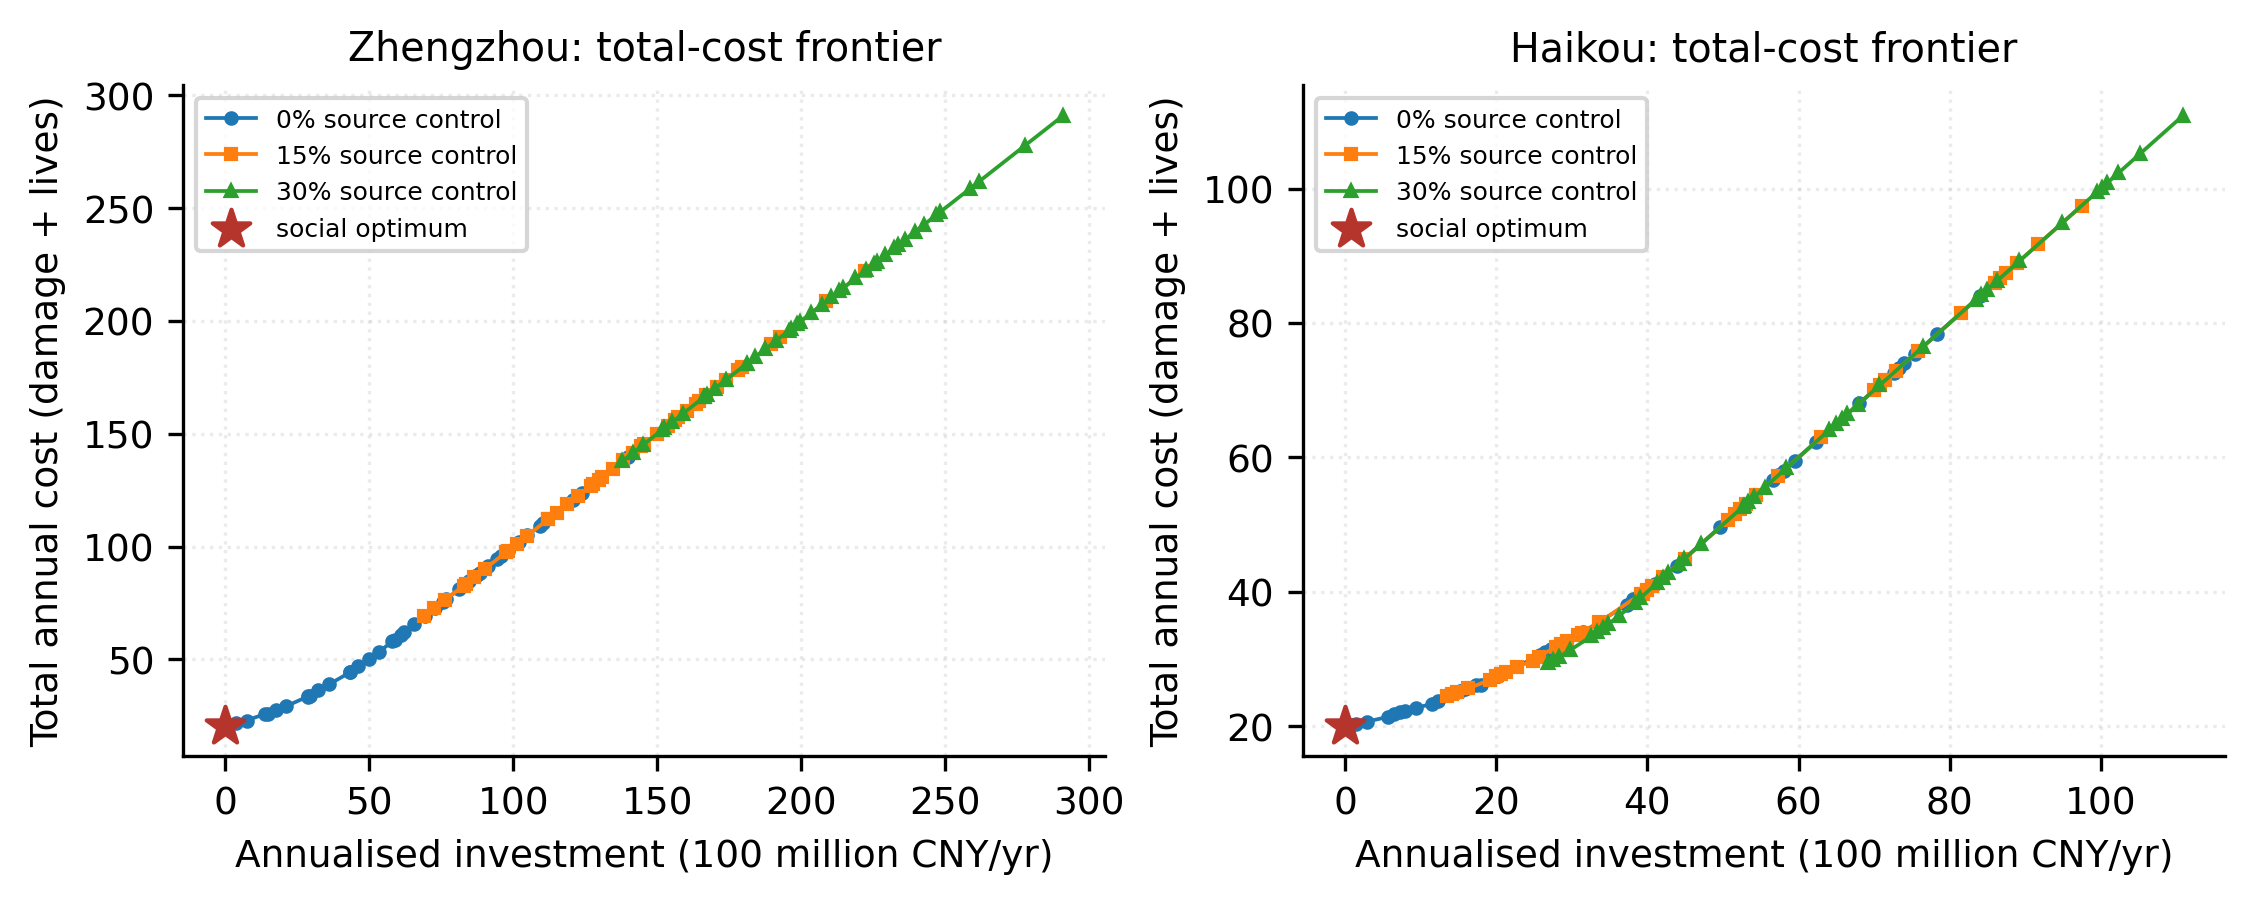
\includegraphics[width=0.60\linewidth]{../02_figures/fig20_cost_damage_frontier.png}
\caption{Total annualised cost (construction amortised over 30 years plus expected residual damage) against annualised investment for Zhengzhou and Haikou. Points on each curve are one plan in the portfolio grid; the star marks the social optimum, not the left edge of the axis.}
\label{fig:frontier}
\end{figure}

\begin{figure}[H]
\centering
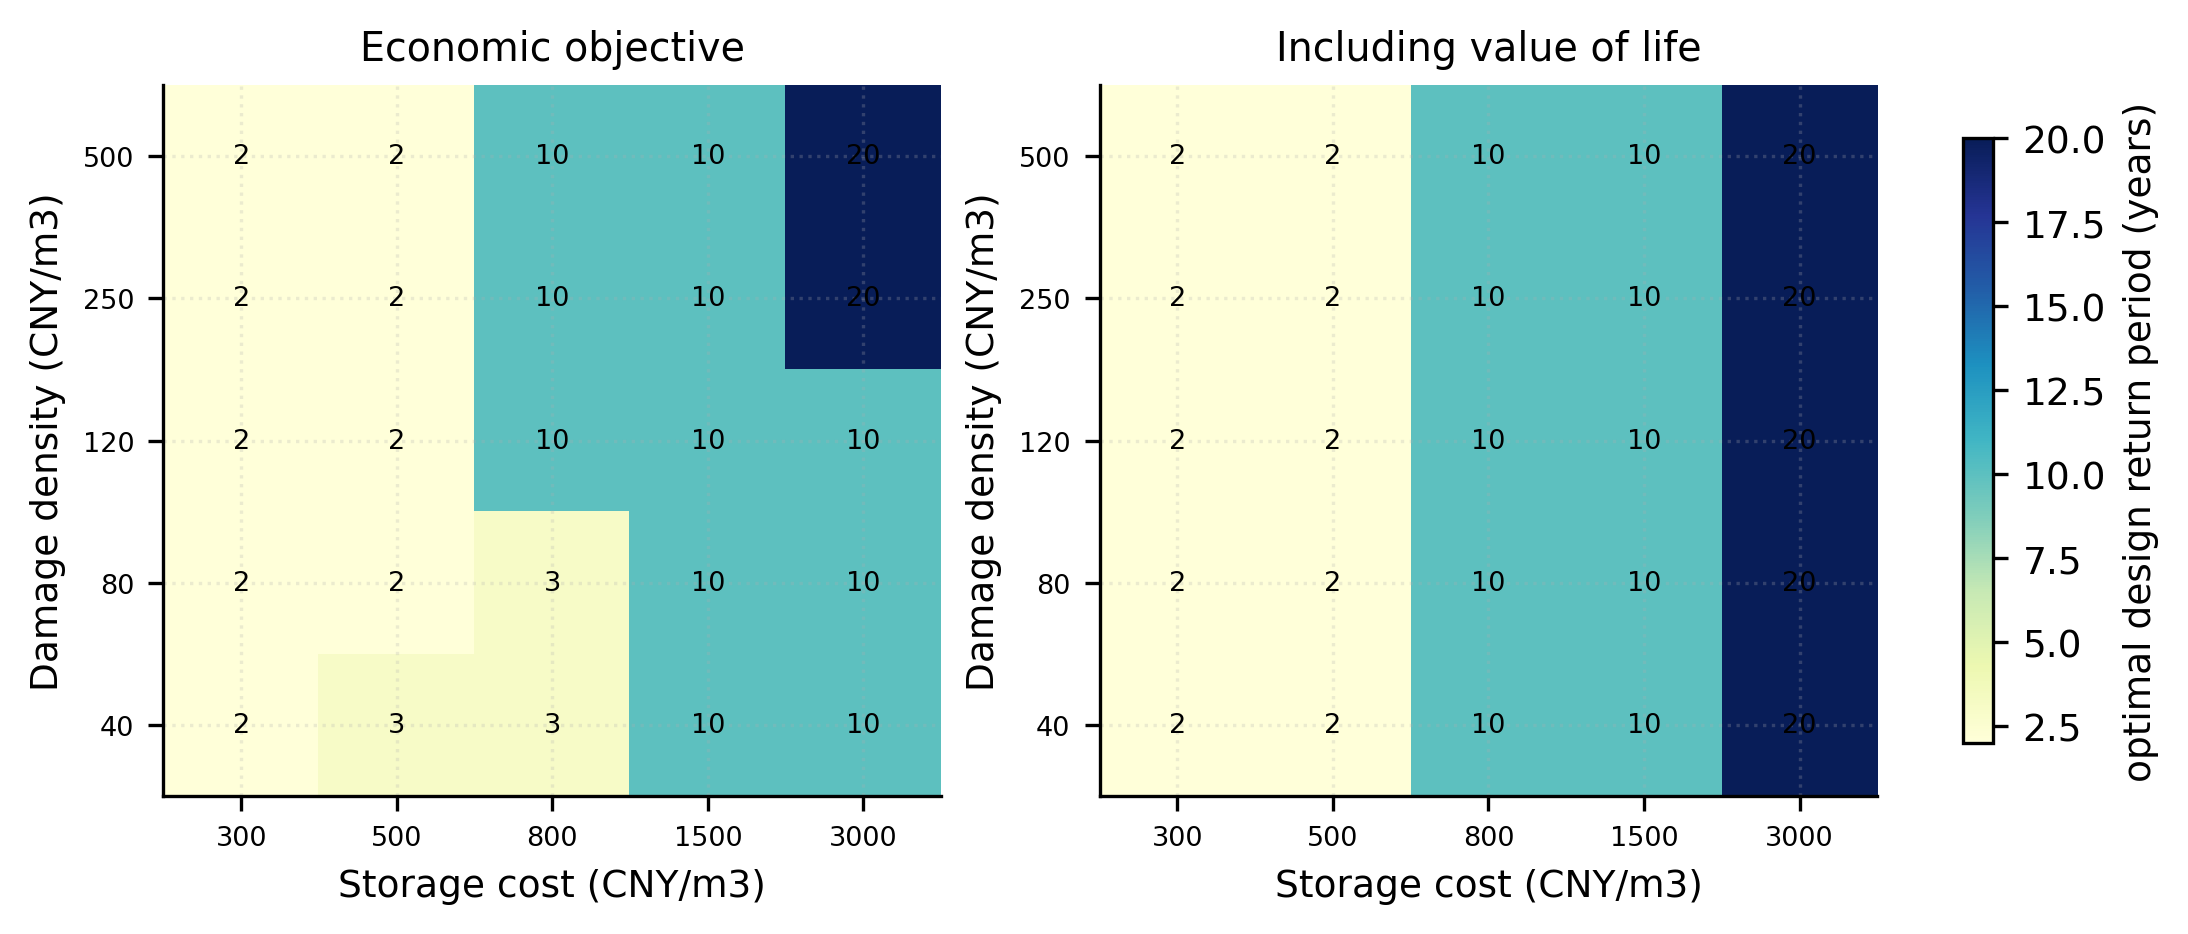
\includegraphics[width=0.60\linewidth]{../02_figures/fig22_sensitivity_tpipe.png}
\caption{Optimal pipe standard against damage density and storage unit cost, under the economic objective (left) and the social objective (right). The standard stays at 2--5 years over most of the space and rises above 10 years only where exposure is extreme and storage expensive.}
\label{fig:senspipe}
\end{figure}